\documentclass[aspectratio=43, dvipsnames]{beamer}
\usepackage[version=4]{mhchem}
\usepackage[aboveskip=1pt, belowskip=1pt]{caption}
\usepackage{amsmath}
\usepackage{siunitx}
\usepackage{emoji}
\usepackage{pgfplots}
\pgfplotsset{compat=1.18,}

% Command to display isotopes
\newcommand{\iso}[2]{\ce{^{#1}#2}}
% Command to write overlap
\newcommand{\overlap}[2]{\left\langle#1\middle\vert#2\right\rangle}
% Command to write Rs
\newcommand{\rs}{$\text{R}_{\text{S}}$ }
% Command to draw enumitems outside the environment
\newcommand{\enumitem}[1]{%
\setcounter{enumi}{#1}\usebeamertemplate{enumerate item}% 
}
\newcommand{\boxitem}[1]{\raisebox{0.15em}{\enumitem{#1}}}
% Set caption package options
\captionsetup{labelformat=empty}

\title[SF quenching]{Quenching of spectroscopic factors in \\ \texorpdfstring{\iso{10,12}{Be}}{10,12Be} transfer reactions}
\date[CPAN]{ASTRANUCAP and CPAN Days 2024}
\author[M. Lozano et al.]{M. Lozano-González, A. Matta, B. Fernández-Domínguez,\texorpdfstring{\newline}{} F. Delaunay, J. Lois-Fuentes}
\institute{USC-IGFAE and LPC-Caen}

\usetheme{igfae}

\begin{document}

\maketitle

\section{Motivation}
\begin{frame}{A recap on spectroscopic factors}
    \textbf{Spectroscopic factors} shed light on the occupancy of single-particle states:
    \begin{equation*}
        \left.\frac{d\sigma}{d\Omega}\right\vert_{\text{exp}} = C^{2}S \cdot \left.\frac{d\sigma}{d\Omega}\right\vert_{\text{s.p}}, \quad \sum C^{2}S = (2j + 1) \text{ in IPSM}
    \end{equation*}
    \begin{columns}[T]
        \begin{column}{0.48\linewidth}
            \hfill{}
            \begin{beamercolorbox}[sep=0.75em, center, wd=0.85\linewidth,rounded=true]{box1}
                \textbf{Experimentally:} Reduction of \sim\qty{65}{\percent}!
            \end{beamercolorbox}%
            \hfill{}
            \begin{itemize}
                \item \textbf{Short-range} correlations: tensor forces,...
                \item \textbf{Long-range}: vibrations, giant resonances,...
            \end{itemize}
        \end{column}
        \begin{column}{0.48\linewidth}
            \vspace{-1em}
            \begin{figure}
                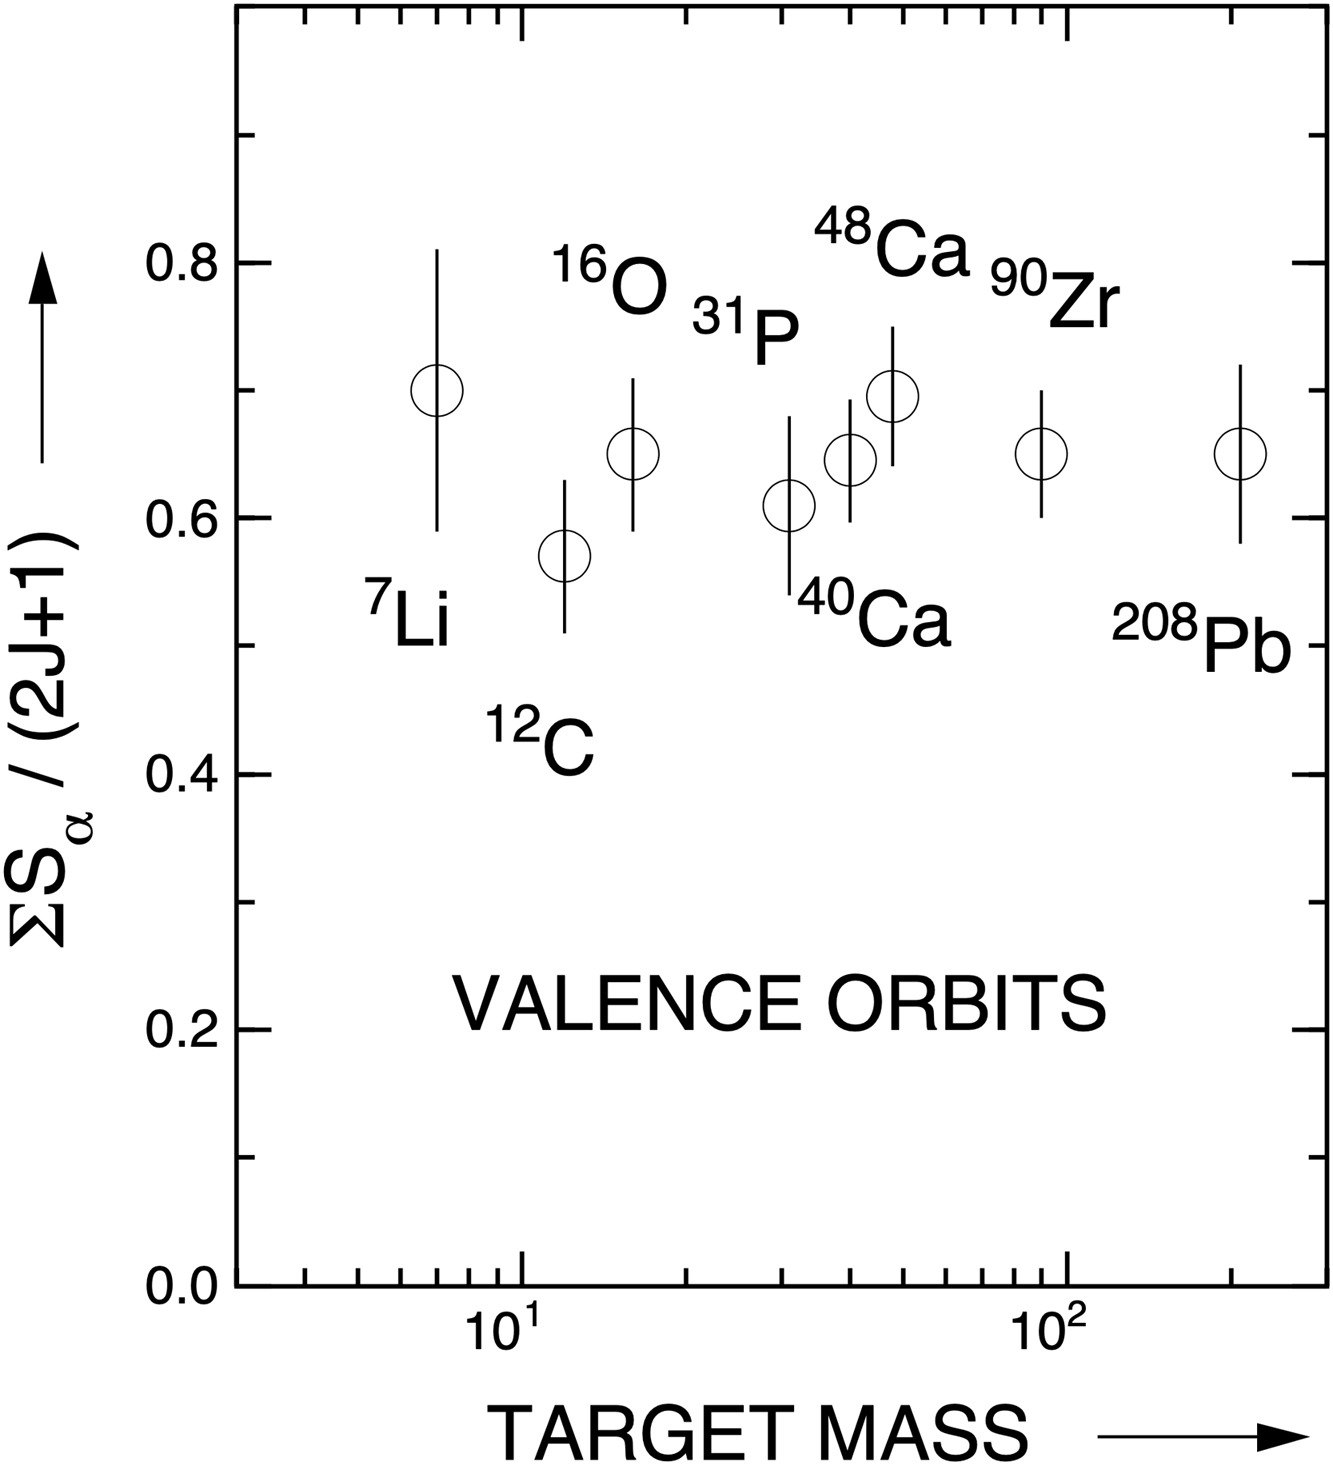
\includegraphics[width=0.725\linewidth]{figures/lapikas_review.jpg}
                \caption{L. Lapikás, Nuclear Phys. A 553 (1993)}
            \end{figure}
        \end{column}
    \end{columns}
\end{frame}

\begin{frame}{A long-standing puzzle}
    A trend with asymmetry energy $\Delta S \equiv \pm \left(S_{p} - S_{n}\right)$ is found depending on the experimental \textbf{probe}!
    \begin{figure}
        \begin{tikzpicture}
            \node[anchor=south west,inner sep=0] (image) at (0,0) { 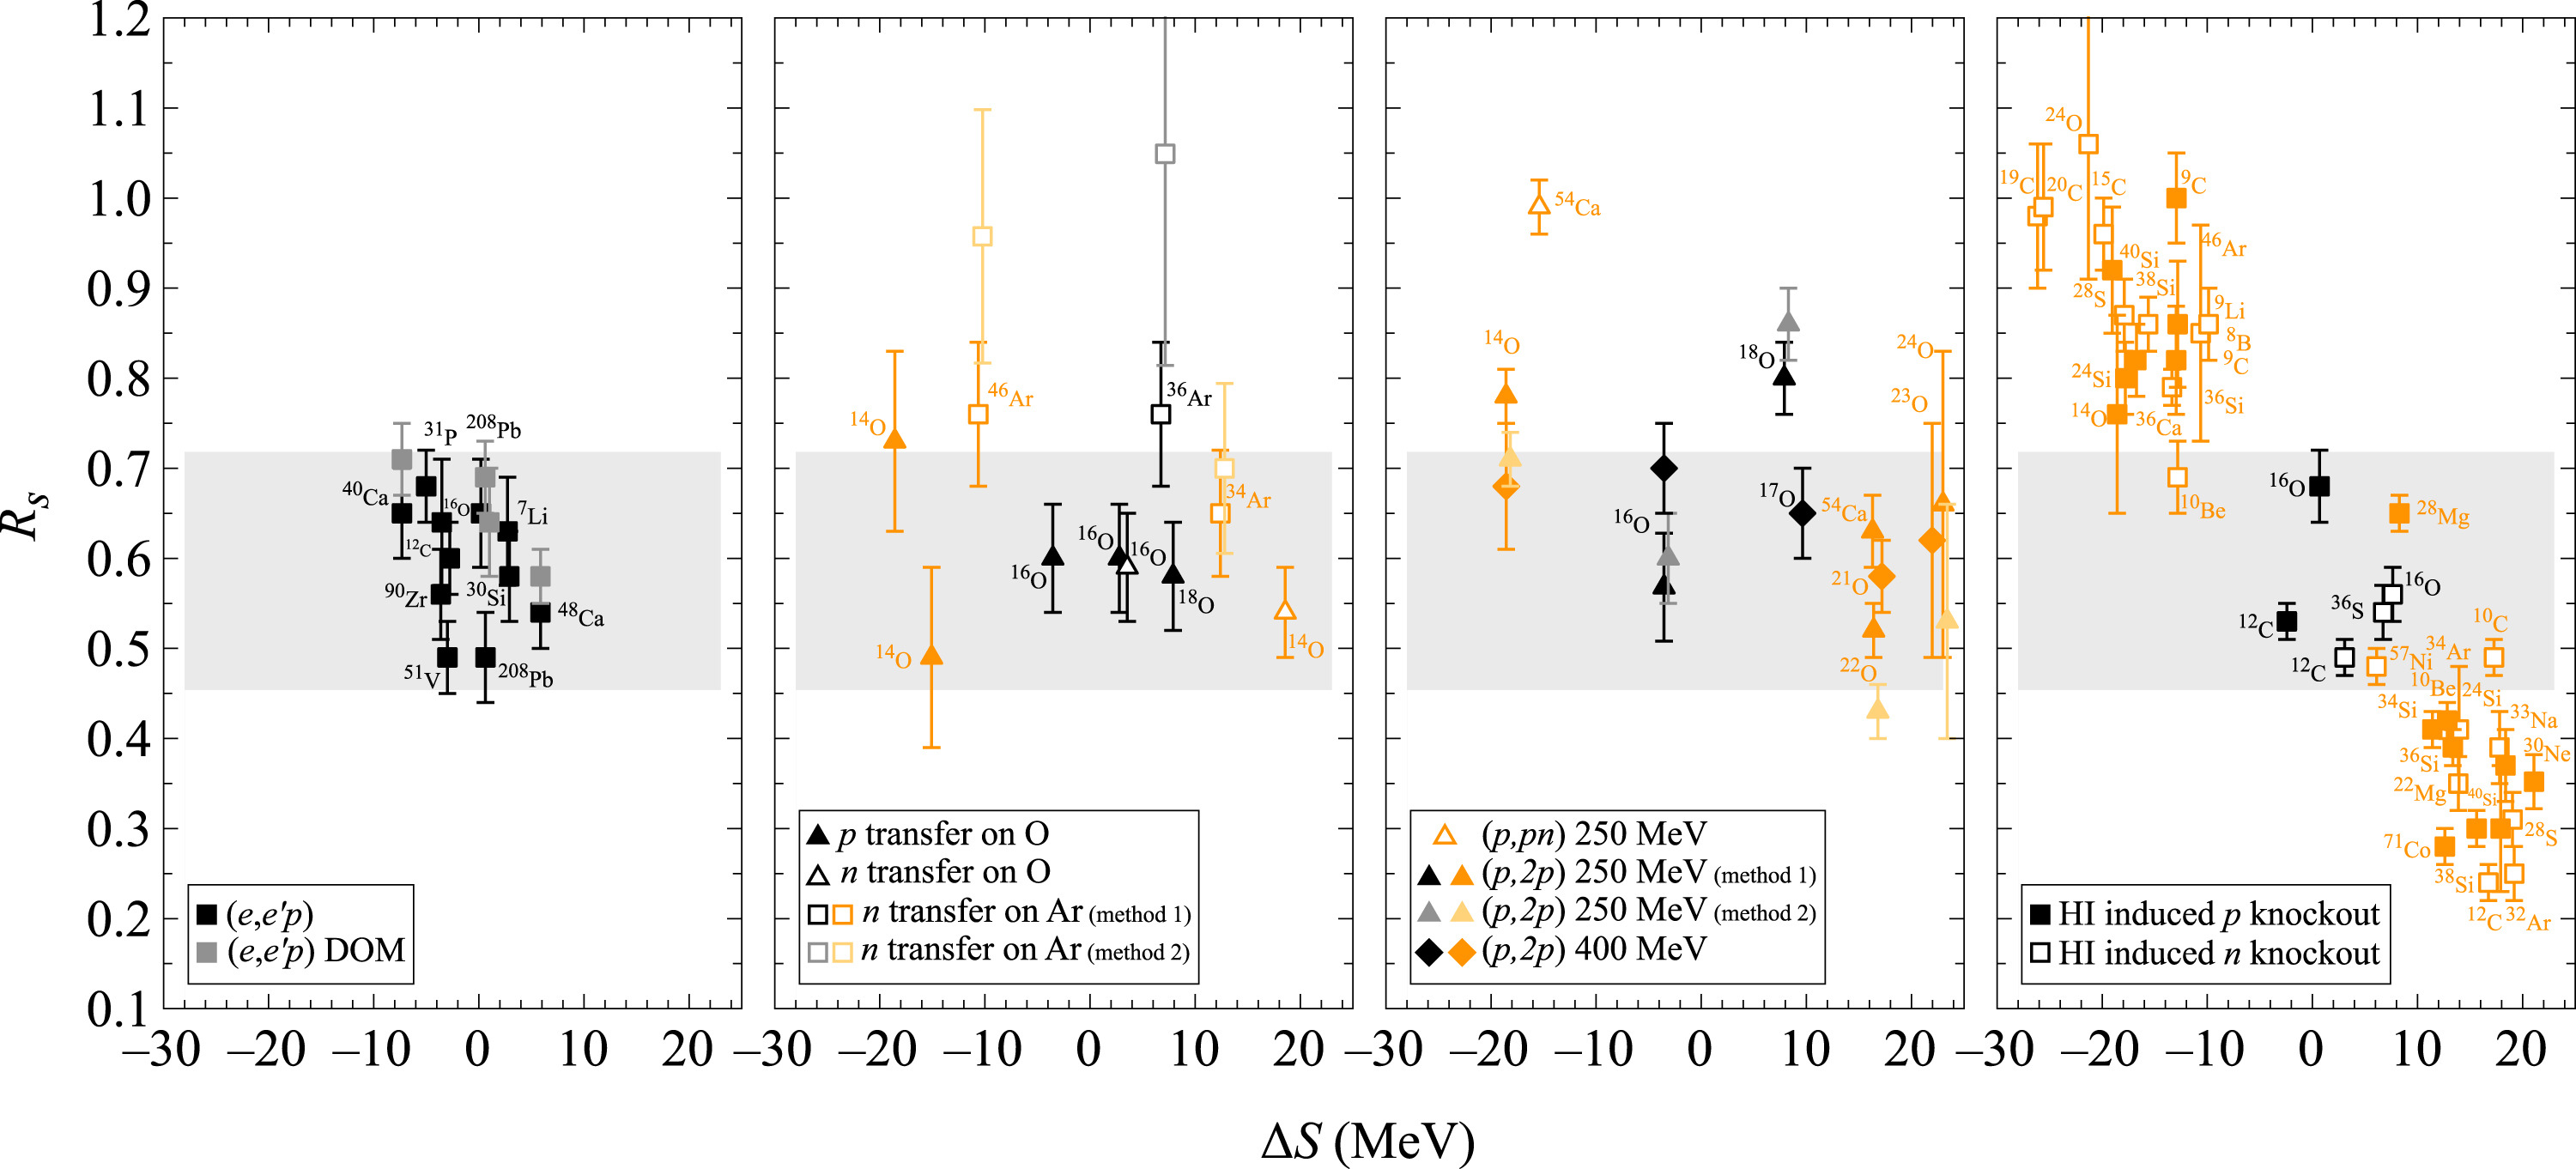
\includegraphics[width=0.9\linewidth]{figures/auman.jpg}
            };
            \myscope[false]{
                \node at (0.17, 0.9) {(e,e'p)};
                \node at (0.405, 0.9) {transfer};
                \node at (0.65, 0.9) {(p,2p)};
                \node[align=center] at (0.89, 0.9) {\textcolor{red}{Be-C} \\ \textcolor{red}{knock-out}};
                \draw[thick, red] (0.825, 0.78) -- (0.97, 0.335);
            }
        \end{tikzpicture}
        \caption{T. Aumann \textit{et al.} Prog. Part. Nucl. Phys. 118 (2021)}
    \end{figure}
    \mycolorbox{box2}{
        $\Rightarrow$ measure towards more exotic nuclei: $\left|\Delta S \right| \uparrow$
    }
\end{frame}

\begin{frame}[t]{Importance of GMF}
    Towards exotic nuclei (loosely bound or halo), a \textbf{\textit{geometrical mismatch factor}} emerges from the very different w.f. in the overlap:
    \vspace{-1em}
    \begin{columns}[T]
        \column{0.48\linewidth}
        {
            \begin{figure}
                \begin{tikzpicture}
                    \node[anchor=south west, inner sep=0pt] (image) at (0,0){
                        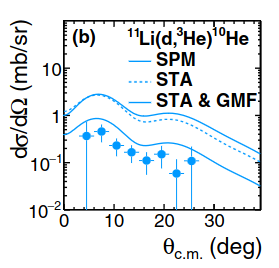
\includegraphics[width=0.7\linewidth]{figures/matta_11Li_d3He.png}};
                    \myscope[false]{
                        \draw[<-, very thick, magenta] (0.6, 0.46) -- (0.68, 0.54);
                        \draw[<-, very thick, magenta] (0.3, 0.55) -- (0.35, 0.65);
                    }
                \end{tikzpicture}
                \caption{A.Matta et al., Phys. Rev. C 92 (2015)}
            \end{figure}
        }
        \column{0.48\linewidth}
        {
            \begin{figure}
                \begin{tikzpicture}
                    \node[anchor=south west, inner sep=0pt] (image) at (0, 0){
                        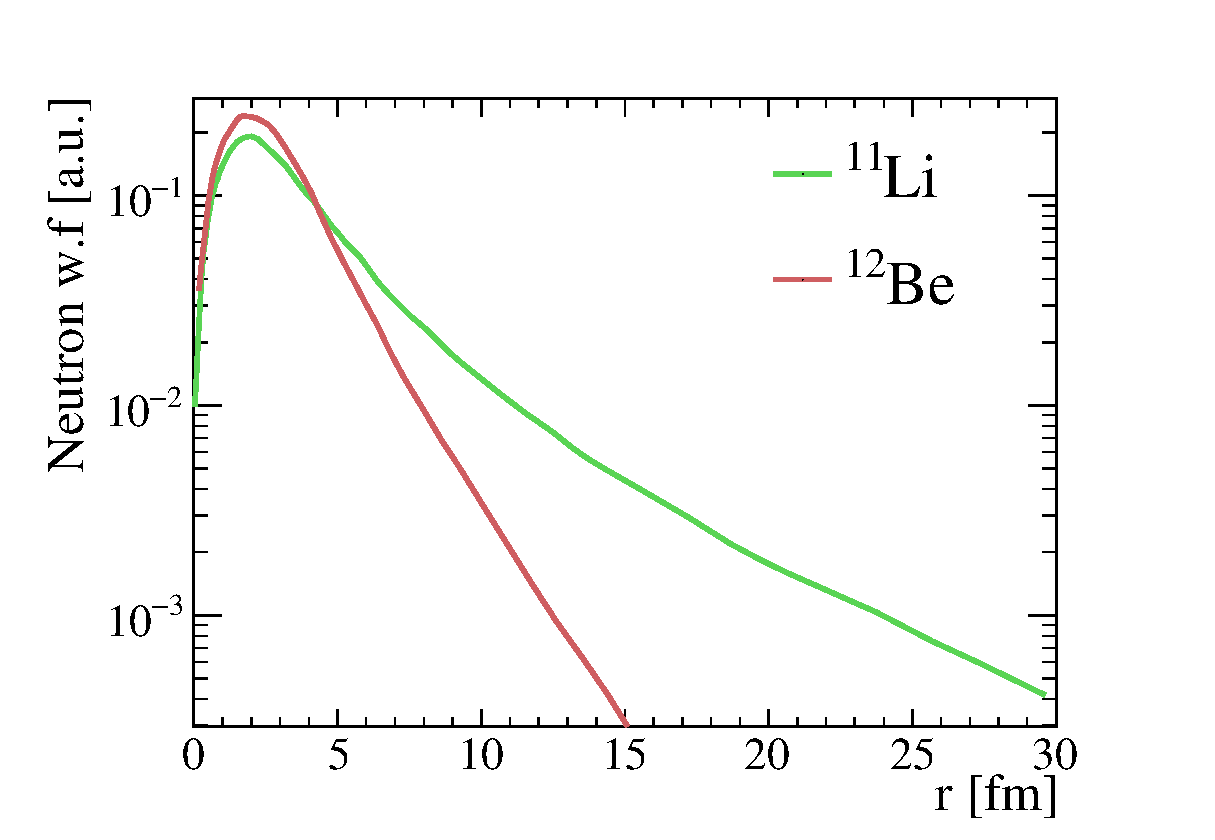
\includegraphics[width=1\linewidth]{figures/wfs.eps}};
                    \myscope[false]{
                        \draw[<->, very thick, dashed, magenta] (0.47, 0.25) -- (0.7, 0.25);
                    }
                \end{tikzpicture}
                \caption{N. K. Timofeyuk, private communication (in E748 proposal)}
            \end{figure}
        }
    \end{columns}
    \begin{columns}[c]
        \begin{column}{0.78\linewidth}
            \mycolorbox[1]{box4}{
                $\Rightarrow$ Need to correct $C^{2}S$ by its value!
            }
        \end{column}
    \end{columns}
\end{frame}

\begin{frame}{Physics case of E748}
    E748 @ GANIL back in 2017. Using \iso{10,12}{Be}(d,t$\vert$\iso{3}{He}) reactions to:
    \bigskip
    \begin{columns}[T]
        \begin{column}{0.52\linewidth}
            \mycolorbox[1]{box2}{
            $\text{R}_{\text{S}}$ and $\Delta S$ dependence:
            {\small
            \begin{itemize}
                \item {\footnotesize $\left\langle\iso{10}{Be}\middle|\iso{9}{Be,Li}\right\rangle$}, $\Delta S = \mp \qty{12.8}{\MeV}$
                \item {\footnotesize $\left\langle\iso{12}{Be}\middle|\iso{11}{Be,Li}\right\rangle$}, $\Delta S = \mp \textcolor{magenta}{\qty{19.8}{\MeV}}$
            \end{itemize}}
            \begin{tikzpicture}[scale=0.95, trim left=-27]
                \begin{axis}[
                    footnotesize,
                    % width=0.5\linewidth,
                    % scale only axis,
                    xlabel={$\Delta$S [MeV]},
                    ylabel={$\text{R}_{\text{S}}$},
                    xmin=-30, xmax=30,
                    ymin=0, ymax=1,
                    ymajorgrids=true, yminorgrids=true,
                    grid style = {dashed},
                    axis on top,
                    ]
                    \addplot[fill=black!12, draw=none, forget plot] coordinates {(\pgfkeysvalueof{/pgfplots/xmin}, 0.45) (\pgfkeysvalueof{/pgfplots/xmax}, 0.45)  (\pgfkeysvalueof{/pgfplots/xmax}, 0.72) (\pgfkeysvalueof{/pgfplots/xmin}, 0.72)};
                    \addplot [orange, only marks,
                        error bars/.cd,
                        y dir=both, y explicit,
                    ] table [row sep=crcr, y error=u] {
                            x		   y      u
                            -18.508    0.732  0.103\\
                            -15.028    0.496  0.099\\
                            -10.552    0.765  0.080\\
                            -3.425    0.607  0.058\\
                            2.873    0.607  0.059\\
                            3.536    0.596  0.060\\
                            6.685    0.765  0.081\\
                            7.845    0.586  0.060\\
                            12.320    0.655  0.072\\
                            18.619    0.546  0.051\\
                        };
                    \draw[black!75, very thick] (axis cs:-12.8,\pgfkeysvalueof{/pgfplots/ymin}) -- (axis cs:-12.8,\pgfkeysvalueof{/pgfplots/ymax});
                    \draw[black!75, very thick] (axis cs:+12.8,\pgfkeysvalueof{/pgfplots/ymin}) -- (axis cs:+12.8,\pgfkeysvalueof{/pgfplots/ymax});
                    \draw[magenta, very thick] (axis cs:-19.8,\pgfkeysvalueof{/pgfplots/ymin}) -- (axis cs:-19.8,\pgfkeysvalueof{/pgfplots/ymax});
                    \draw[magenta, very thick] (axis cs:+19.8,\pgfkeysvalueof{/pgfplots/ymin}) -- (axis cs:+19.8,\pgfkeysvalueof{/pgfplots/ymax});
                    \node[right] at (-12.8, 0.4) {\iso{10}{Be}};
                    \node[magenta, right] at (-20.8, 0.25) {\iso{12}{Be}};
                \end{axis}
            \end{tikzpicture}
            }
        \end{column}
        \begin{column}{0.48\linewidth}
            \mycolorbox[1]{box3}{\small
                Explore effects of GMF:
                \begin{itemize}
                    \item $\left\langle\iso{10}{Be}\middle|\iso{9}{Be,Li}\right\rangle, \text{GMF} \sim \num{1}$
                    \item $\left\langle\iso{12}{Be}\middle|\iso{11}{Li}\right\rangle, \text{GMF} \sim \textcolor{blue}{\num{0.5}?}$
                \end{itemize}
                \begin{tikzpicture}[
                        trim left=-27,
                    ]
                    \centering
                    \begin{axis}[
                        width=0.63\linewidth,
                        scale only axis,
                        ylabel={$\text{S}_{\text{2n}}$ [MeV]},
                        xticklabels={\iso{10}{Be}, \iso{9}{Li}, \iso{12}{Be}, \textcolor{magenta}{\iso{11}{Li}}},
                        xtick={1,2,3, 4},
                        xmin=0.75, xmax=4.25,
                        ymin=0, ymax=8.5,
                        ymajorgrids=true, yminorgrids=true,
                        % ytick distance=0.25,
                        grid style = {dashed},
                        % x tick label style = {font=\tiny},
                        ]
                        \addplot+ [
                            scatter/classes={
                                    a={blue},
                                    b={magenta}
                                },
                            scatter,
                            scatter src=explicit symbolic,
                        ] coordinates {
                                (1, 8.48) [a]
                                (2, 6.10) [a]
                                (3, 3.67) [a]
                                (4, 0.37) [b]
                            };
                    \end{axis}
                \end{tikzpicture}
            }
        \end{column}
    \end{columns}
\end{frame}

\section{Methodology}
\begin{frame}[c]{Experimental technique}
    Tradional solid target experiment @ LISE
    \vspace{1.5em}
    \begin{tikzpicture}
        \node[anchor=south west, inner sep = 0pt] (image) at (0,0){
            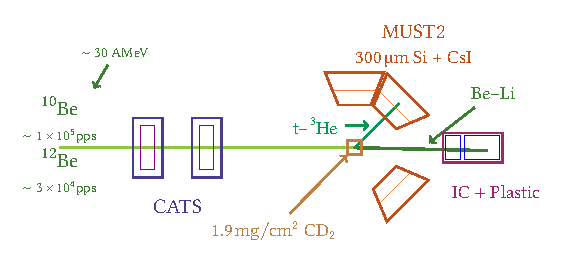
\includegraphics[width=1\linewidth]{figures/setup.pdf}
        };
        \myscope[false]{
            \node at(0.3, -0.15) {
                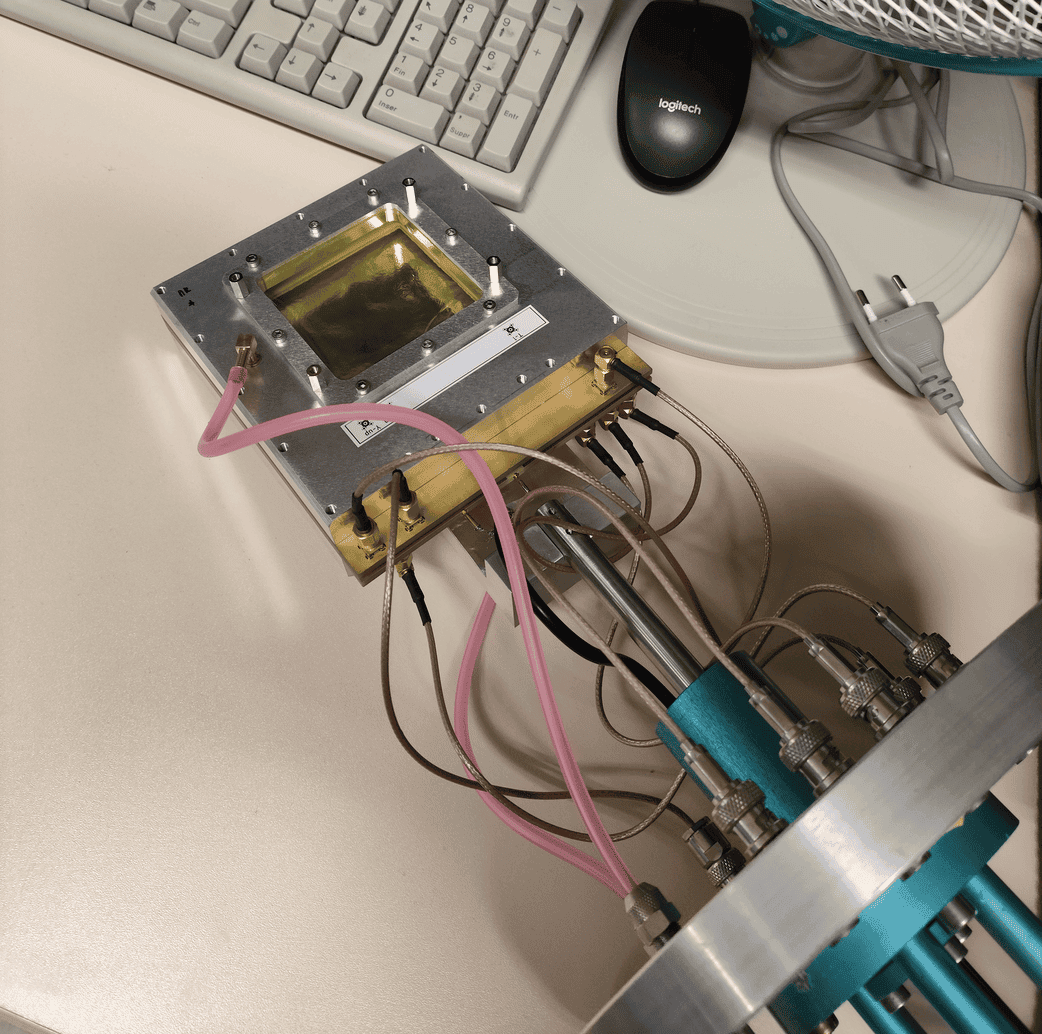
\includegraphics[width=0.22\linewidth]{figures/cats_pic_e870.png}
            };
            \node at(0.8, -0.12) {
                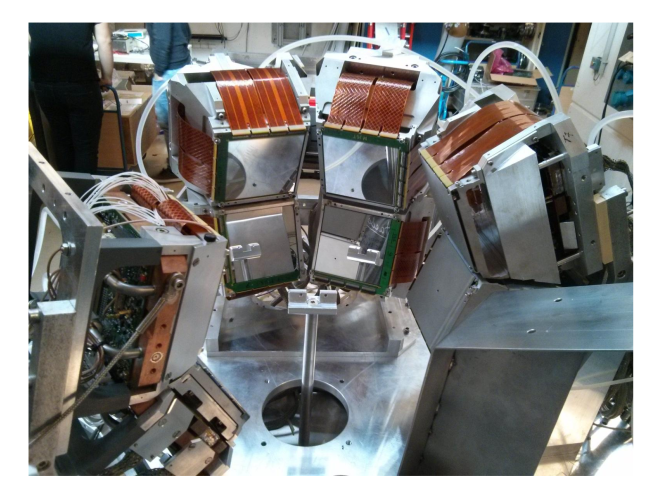
\includegraphics[width=0.35\linewidth]{figures/must2_pic.png}
            };
        }
    \end{tikzpicture}
\end{frame}

\begin{frame}[t]{A glance at the analysis}
    \begin{columns}[T]
        \begin{column}{0.48\linewidth}
            \mycolorbox{box4}{
                \enumitem{1} \textbf{Heavy} ID at \qty{0}{\degree}
            }
            \begin{tikzpicture}
                \node[anchor = south west, inner sep = 0pt] (image) at (0,0){
                    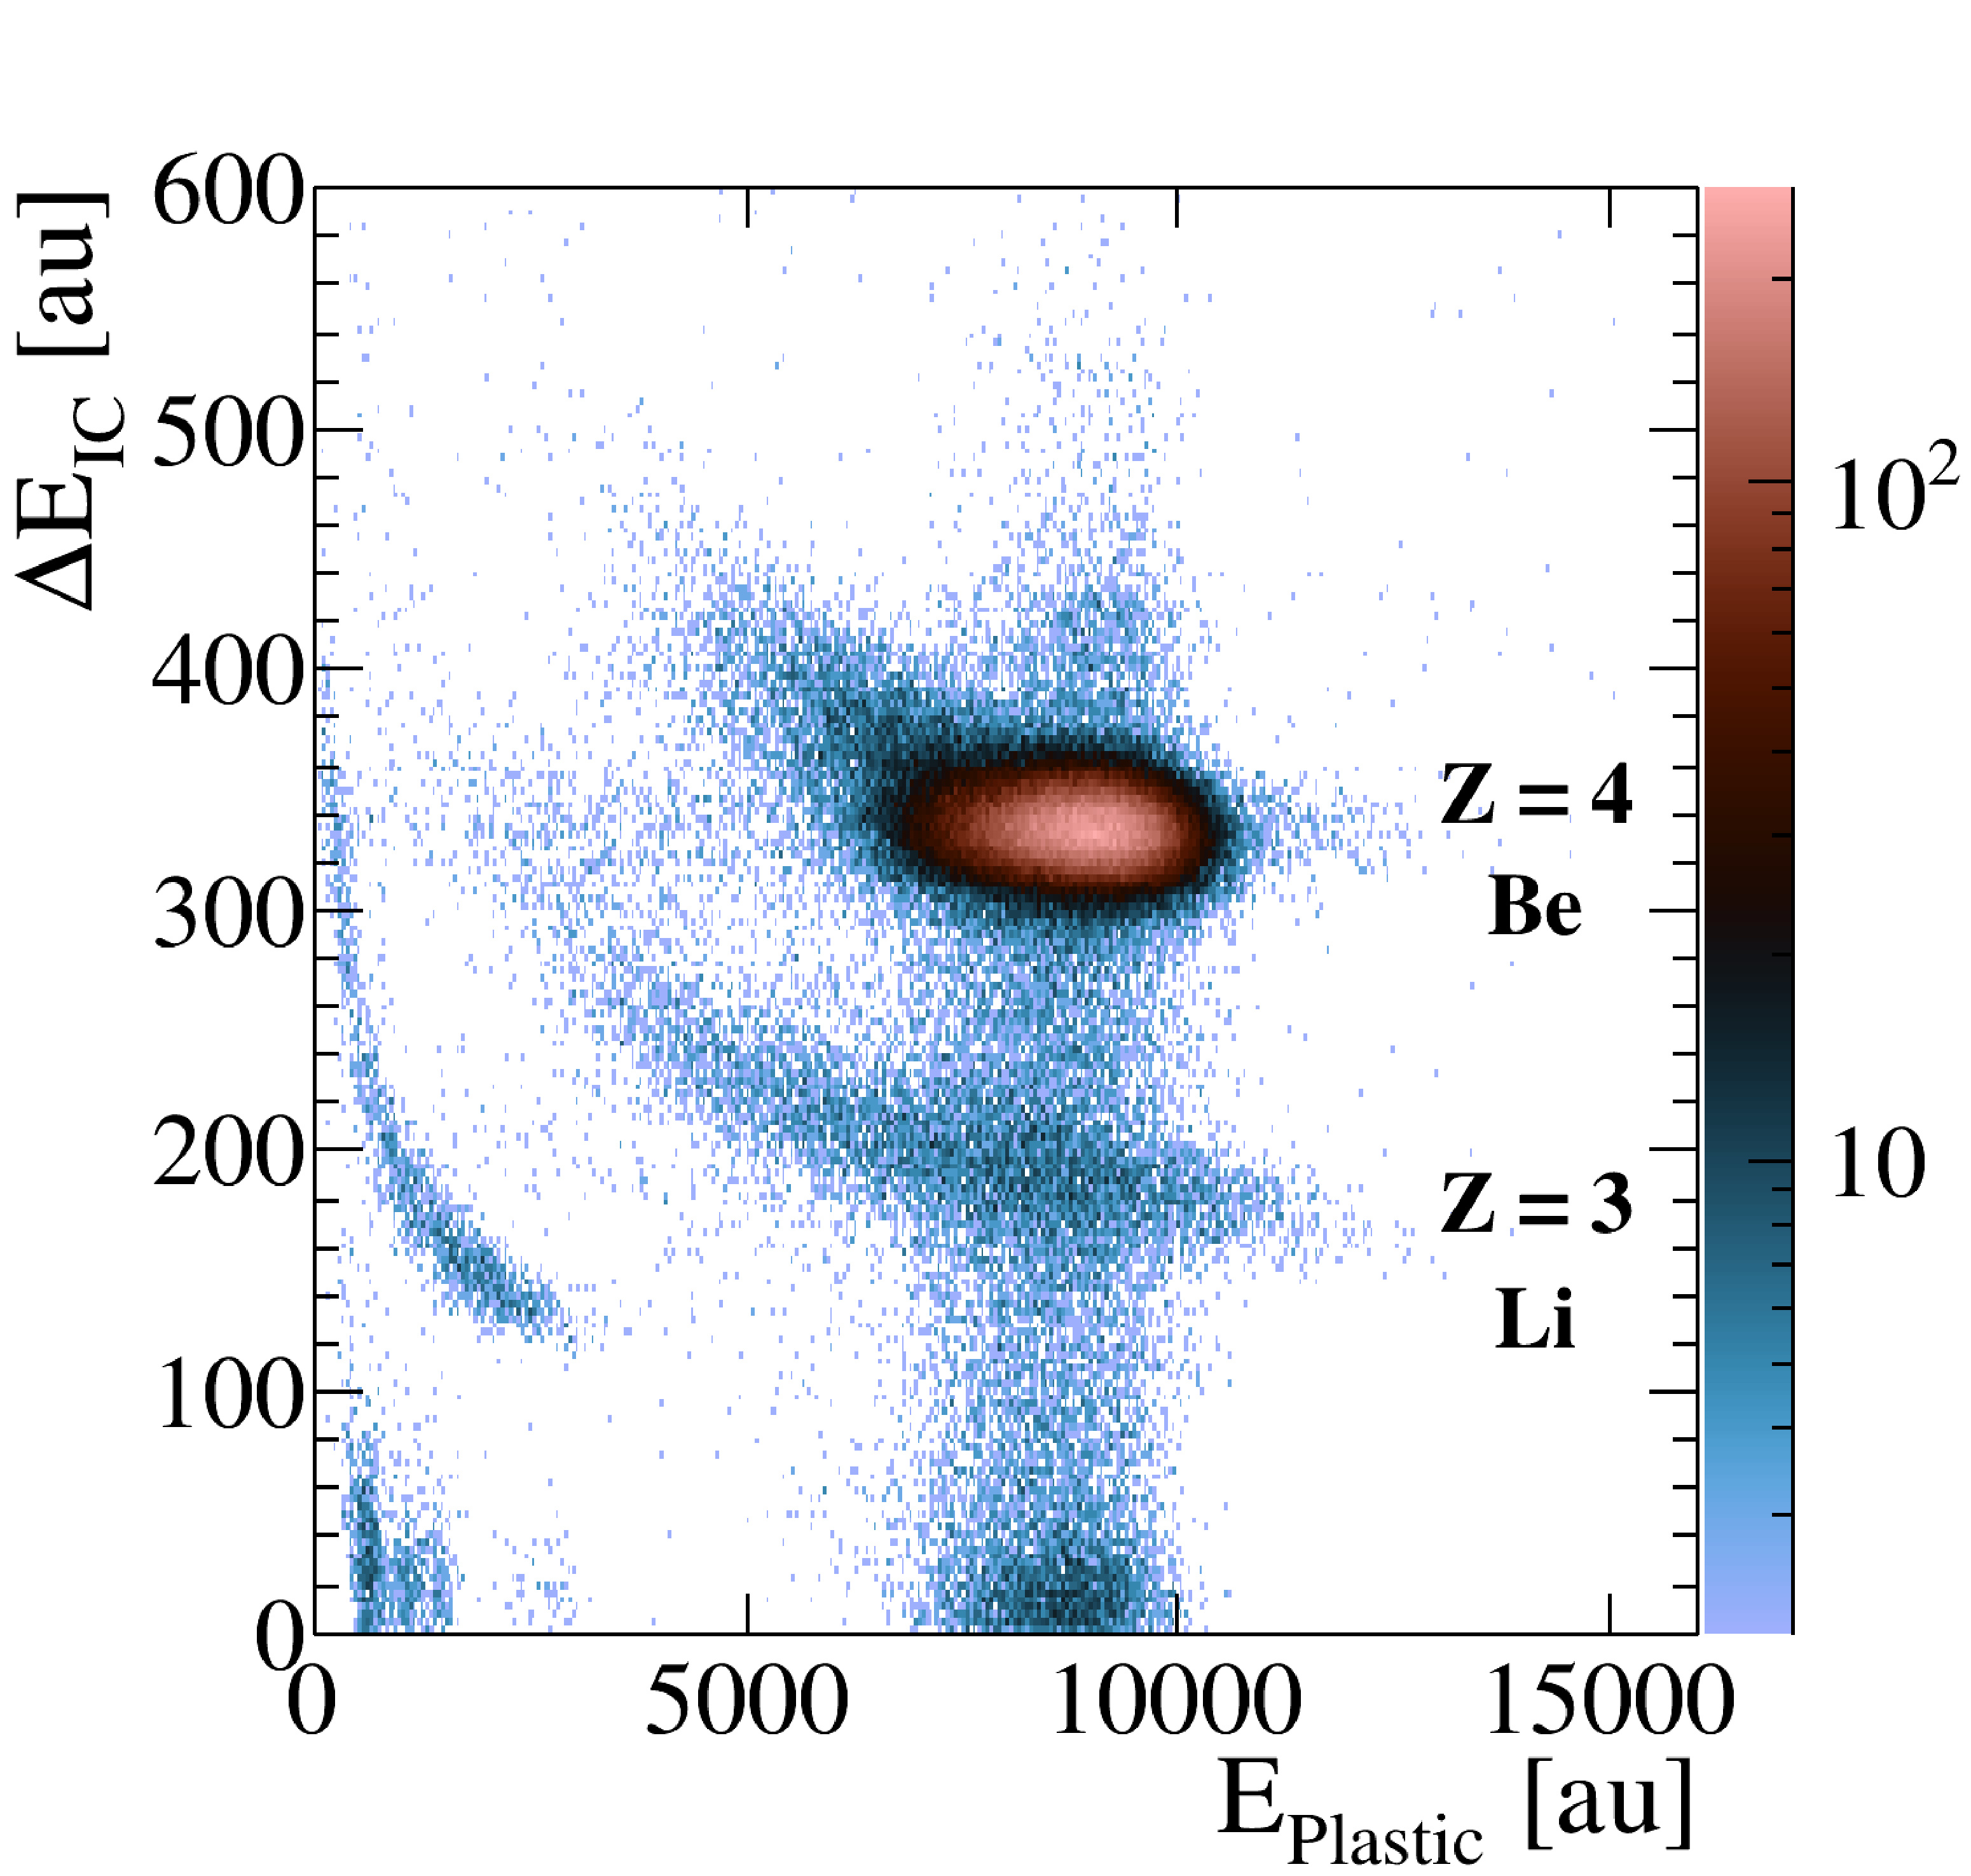
\includegraphics[width=1\linewidth]{figures/heavy.pdf}
                };
            \end{tikzpicture}
        \end{column}
        \begin{column}{0.48\linewidth}
            \mycolorbox{box2}{
                \enumitem{2} \textbf{Light} PID in DSSD
            }
            \begin{tikzpicture}
                \node[anchor = south west, inner sep = 0pt] (image) at (0,0){
                    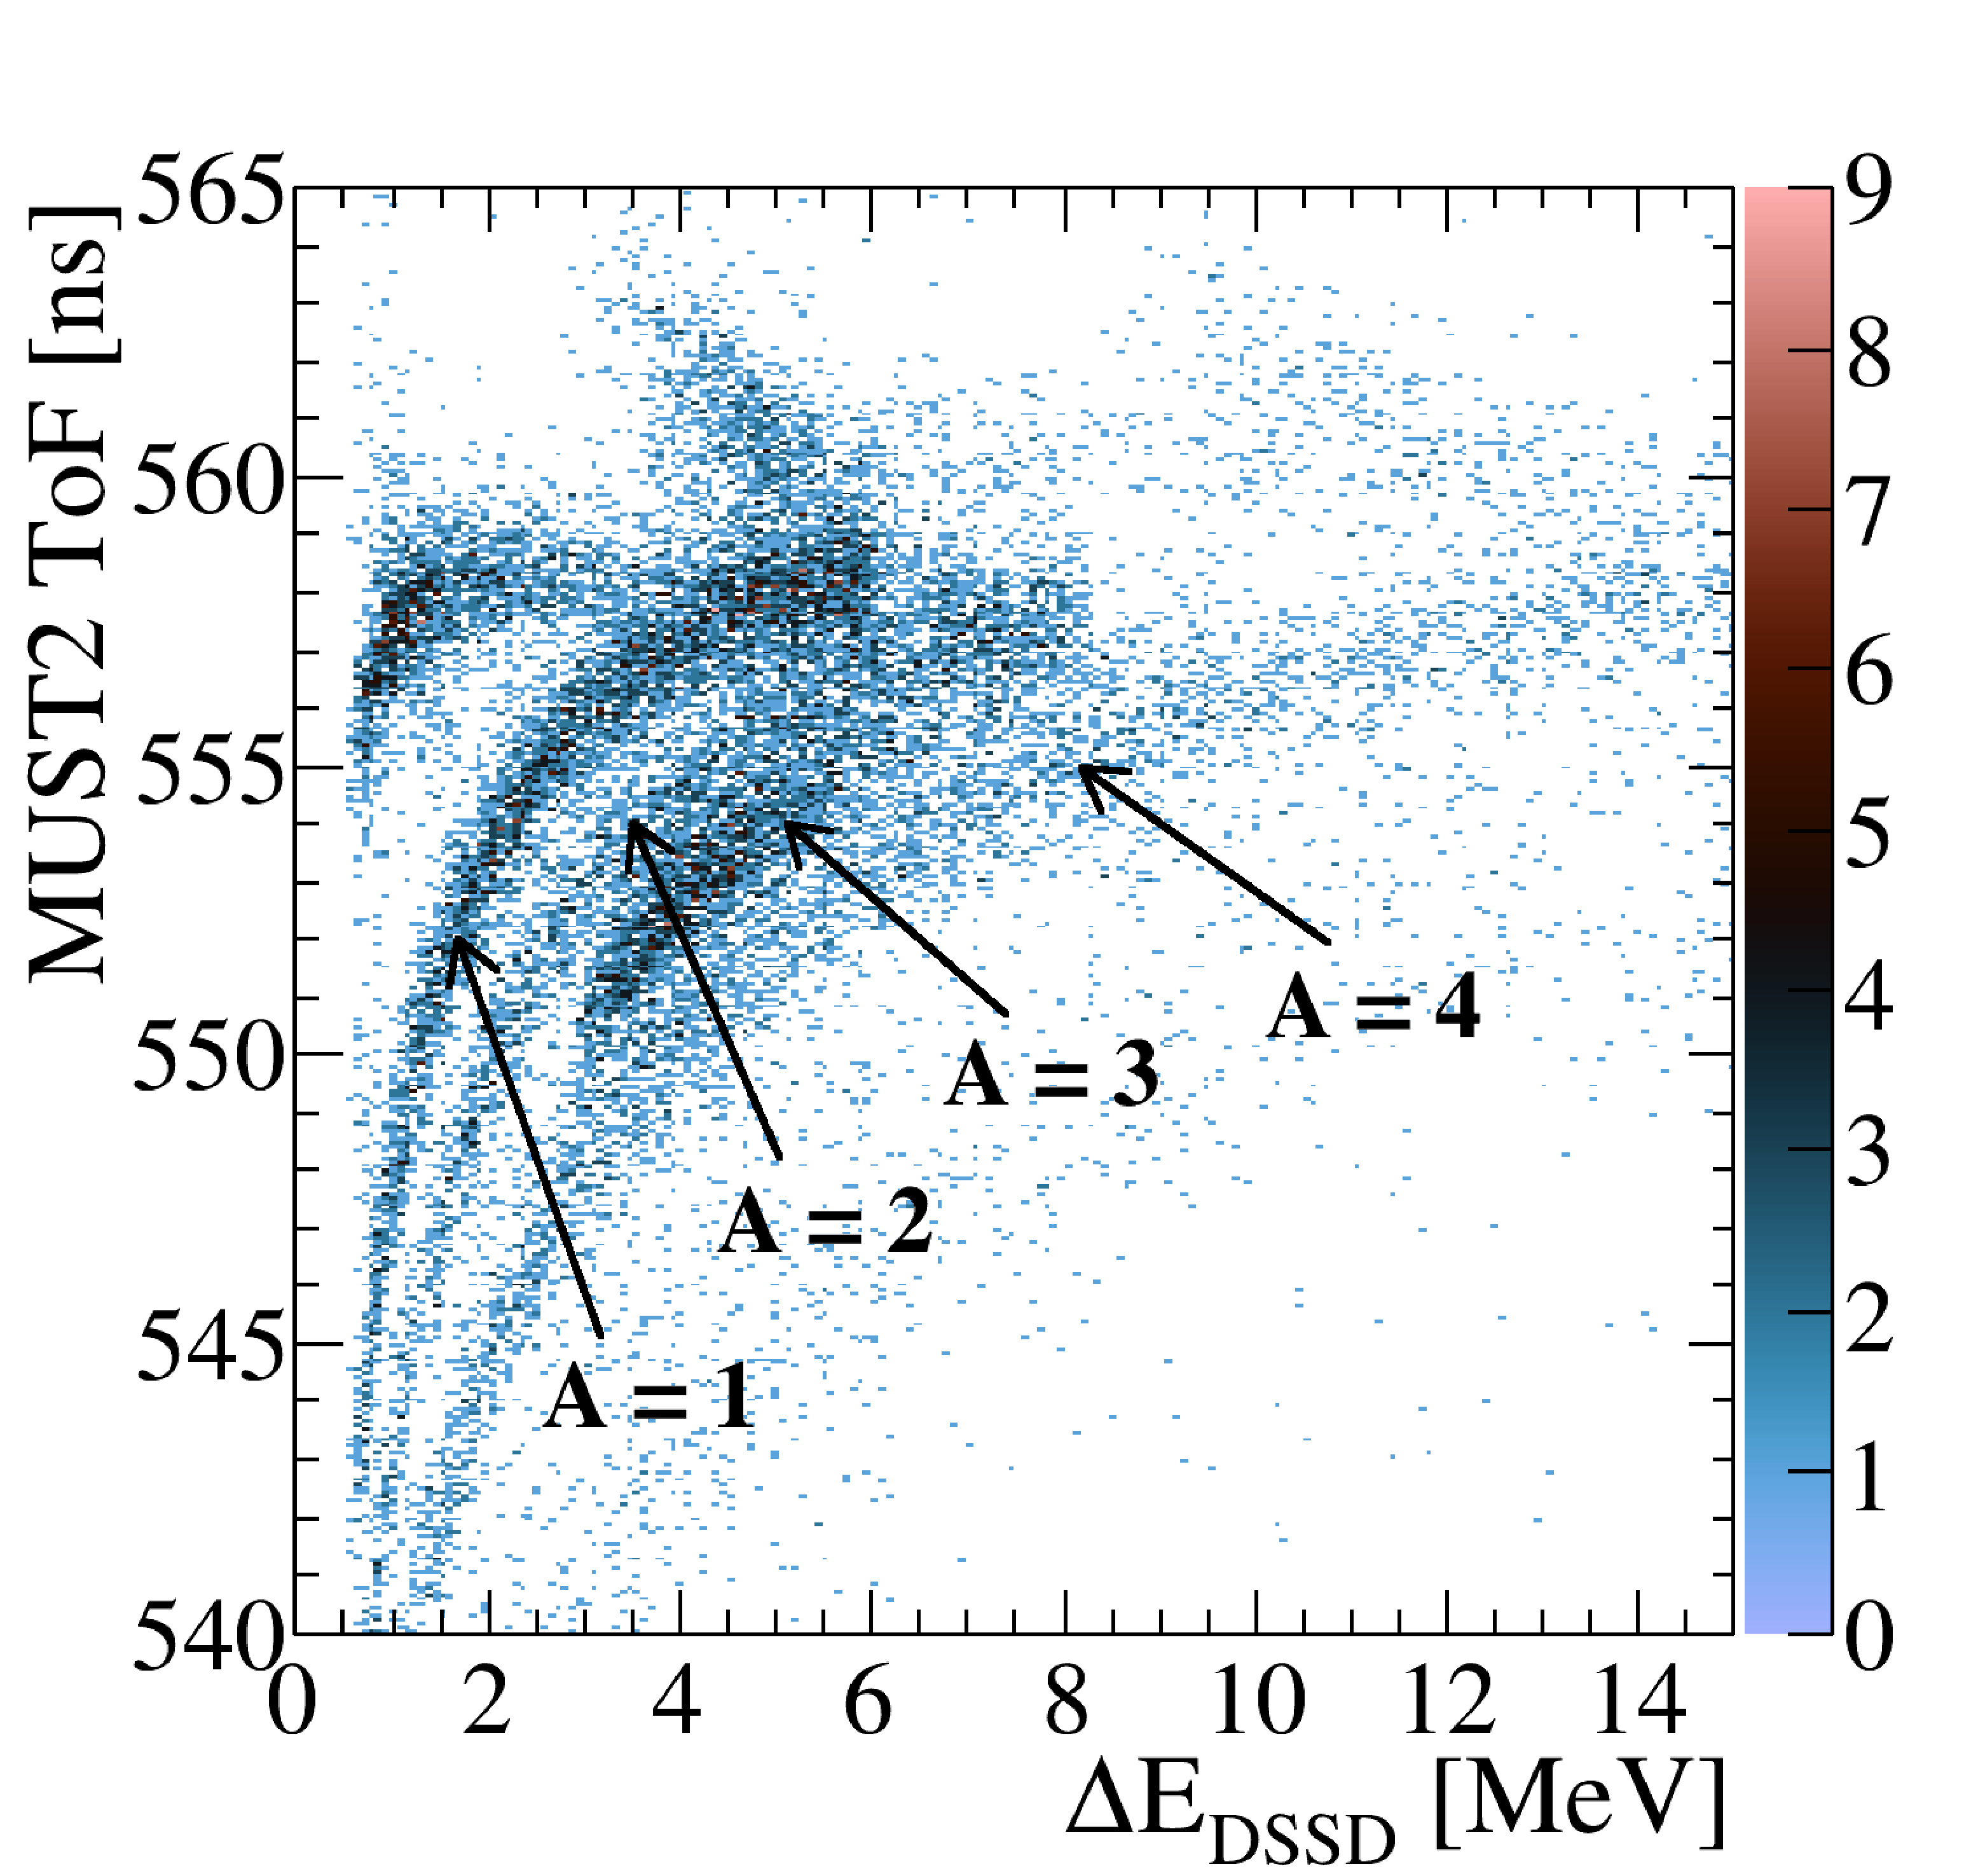
\includegraphics[width=1\linewidth]{figures/light.pdf}
                };
            \end{tikzpicture}
        \end{column}
    \end{columns}
    \mycolorbox{box1}{
        \enumitem{3} $E_{x}$ from \textbf{missing mass technique}
        $E_{\textrm{beam}} + (E,\theta)_{\textrm{Lab}} \rightarrow E_{x}$
    }
\end{frame}

\section{Results}
\begin{frame}[c]{Results: Elastic \texorpdfstring{\iso{10,12}{Be}(d,d)\iso{10,12}{Be} }{10,12Be(d,d)10,12Be}}
    \only<+>{
        The \textbf{ground state} sets our normalization!
        \begin{figure}
            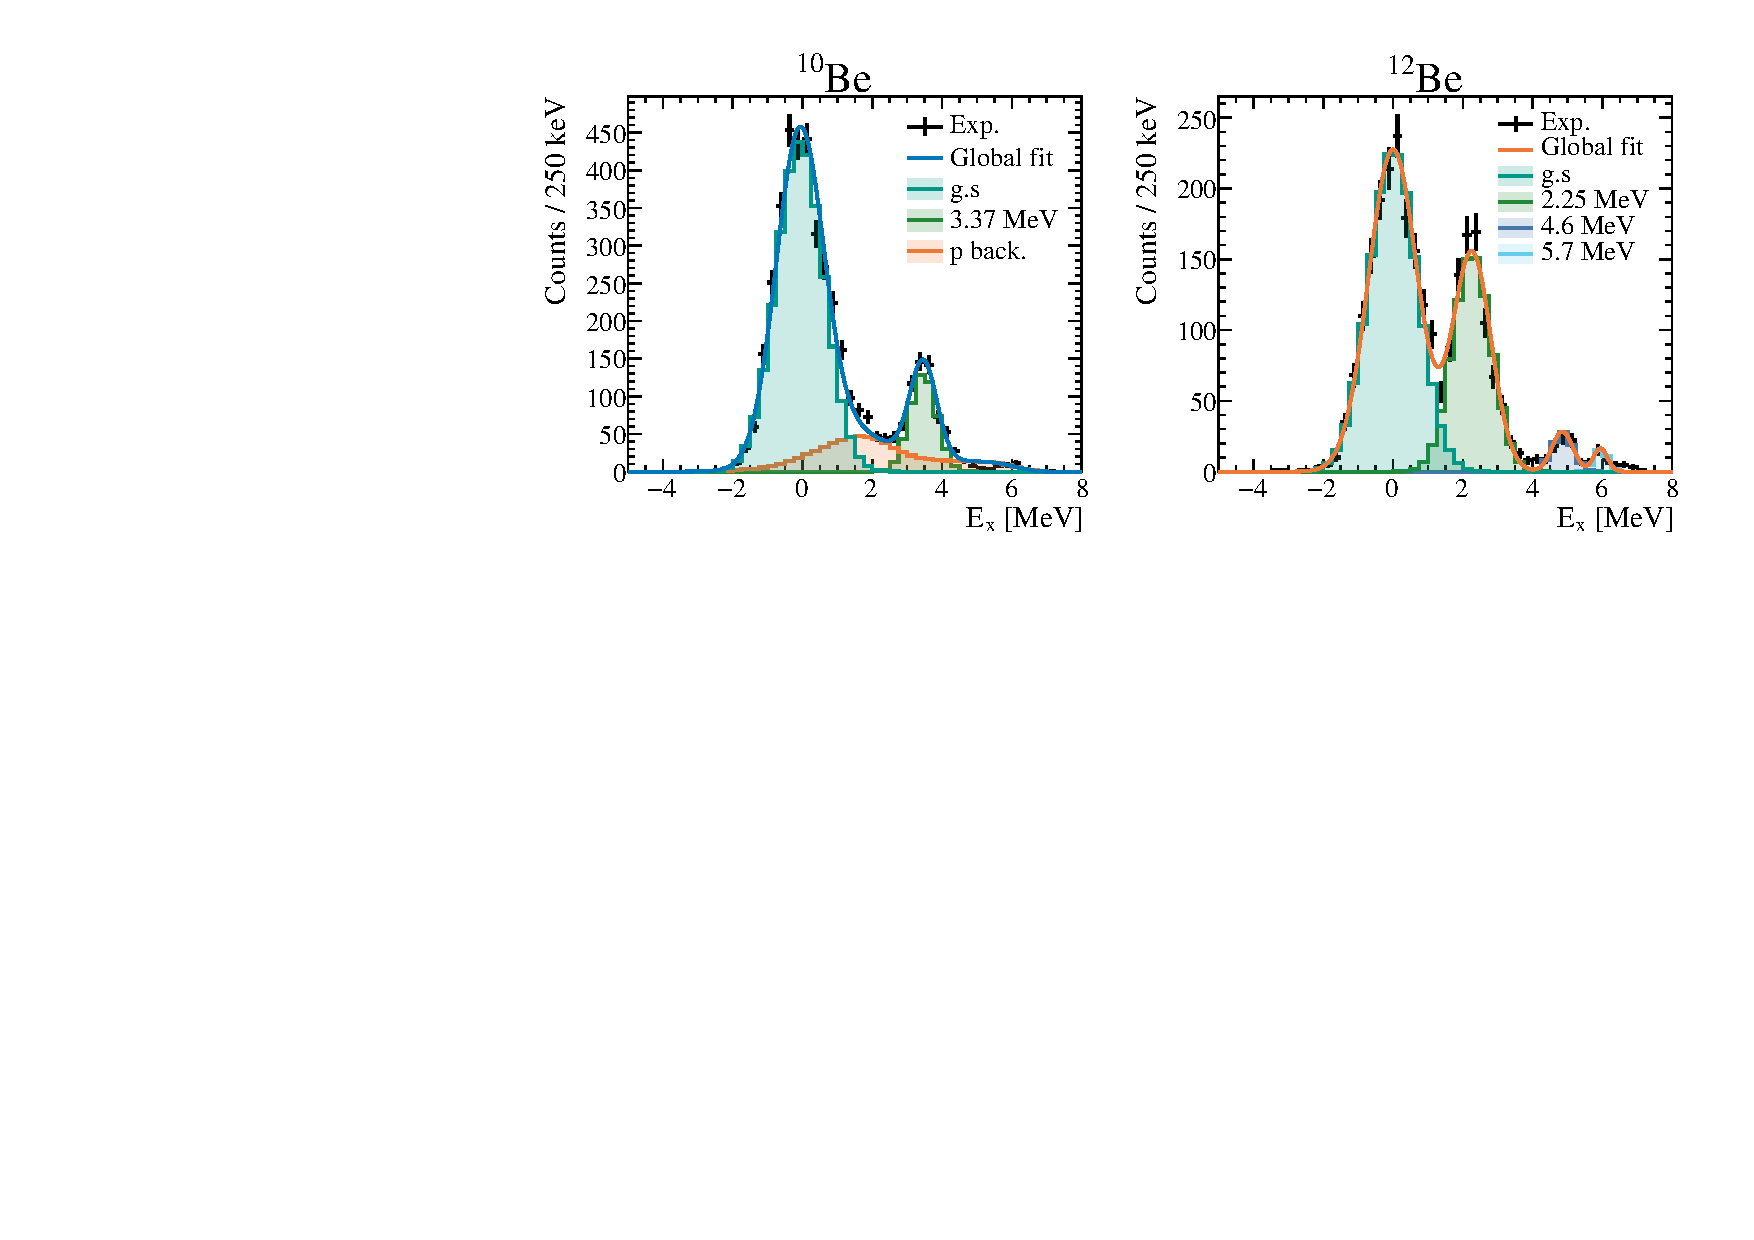
\includegraphics[width=1\linewidth]{figures/elastic_ex.pdf}
        \end{figure}
        \mycolorbox{box2}{
            First $2^{+}$ is seen in both cases but not yet exploited!}
    }
    \only<+>{
        Experimental cross-section formula:
        \begin{equation*}
            \frac{d\sigma}{d\Omega} = \frac{N}{N_{\text{beam}} \textcolor{red}{N_{\text{targets}}} \textcolor{red}{\epsilon} \Delta \Omega} = \frac{N}{N_{\text{beam}} \textcolor{red}{\alpha} \epsilon_{\text{sim}} \Delta \Omega}
        \end{equation*}
        \begin{columns}[c]
            \begin{column}{0.5\linewidth}
                \mycolorbox[1]{box2}{
                    \enumitem{1} \textbf{Target thickness} not measured during experiment:
                    \begin{itemize}
                        \item Set it from normalization of elastic
                    \end{itemize}}
            \end{column}%
            \begin{column}{0.5\linewidth}
                \mycolorbox[1]{box4}{
                    \enumitem{2} ZDD had a poor performance.
                    \begin{itemize}
                        \item Estimated $\sim$ \qtyrange[range-phrase={\text{--}}, range-units=single]{20}{30}{\percent}
                    \end{itemize}}
            \end{column}
        \end{columns}
        \mycolorbox[1]{box3}{
            Agglutination of unknown factors: $\alpha = N_{\text{targets}} \cdot \epsilon_{\text{instrinsic, ZDD}}$
        }
        \vspace{-0.35em}
        \mycolorbox[1]{box1}{
            $\alpha$ is determined from fits of theoretical cross-sections to data
        }
    }%
    \only<+>{
        The best OMP potentials can also be deduced from the fit quality.
        \begin{figure}
            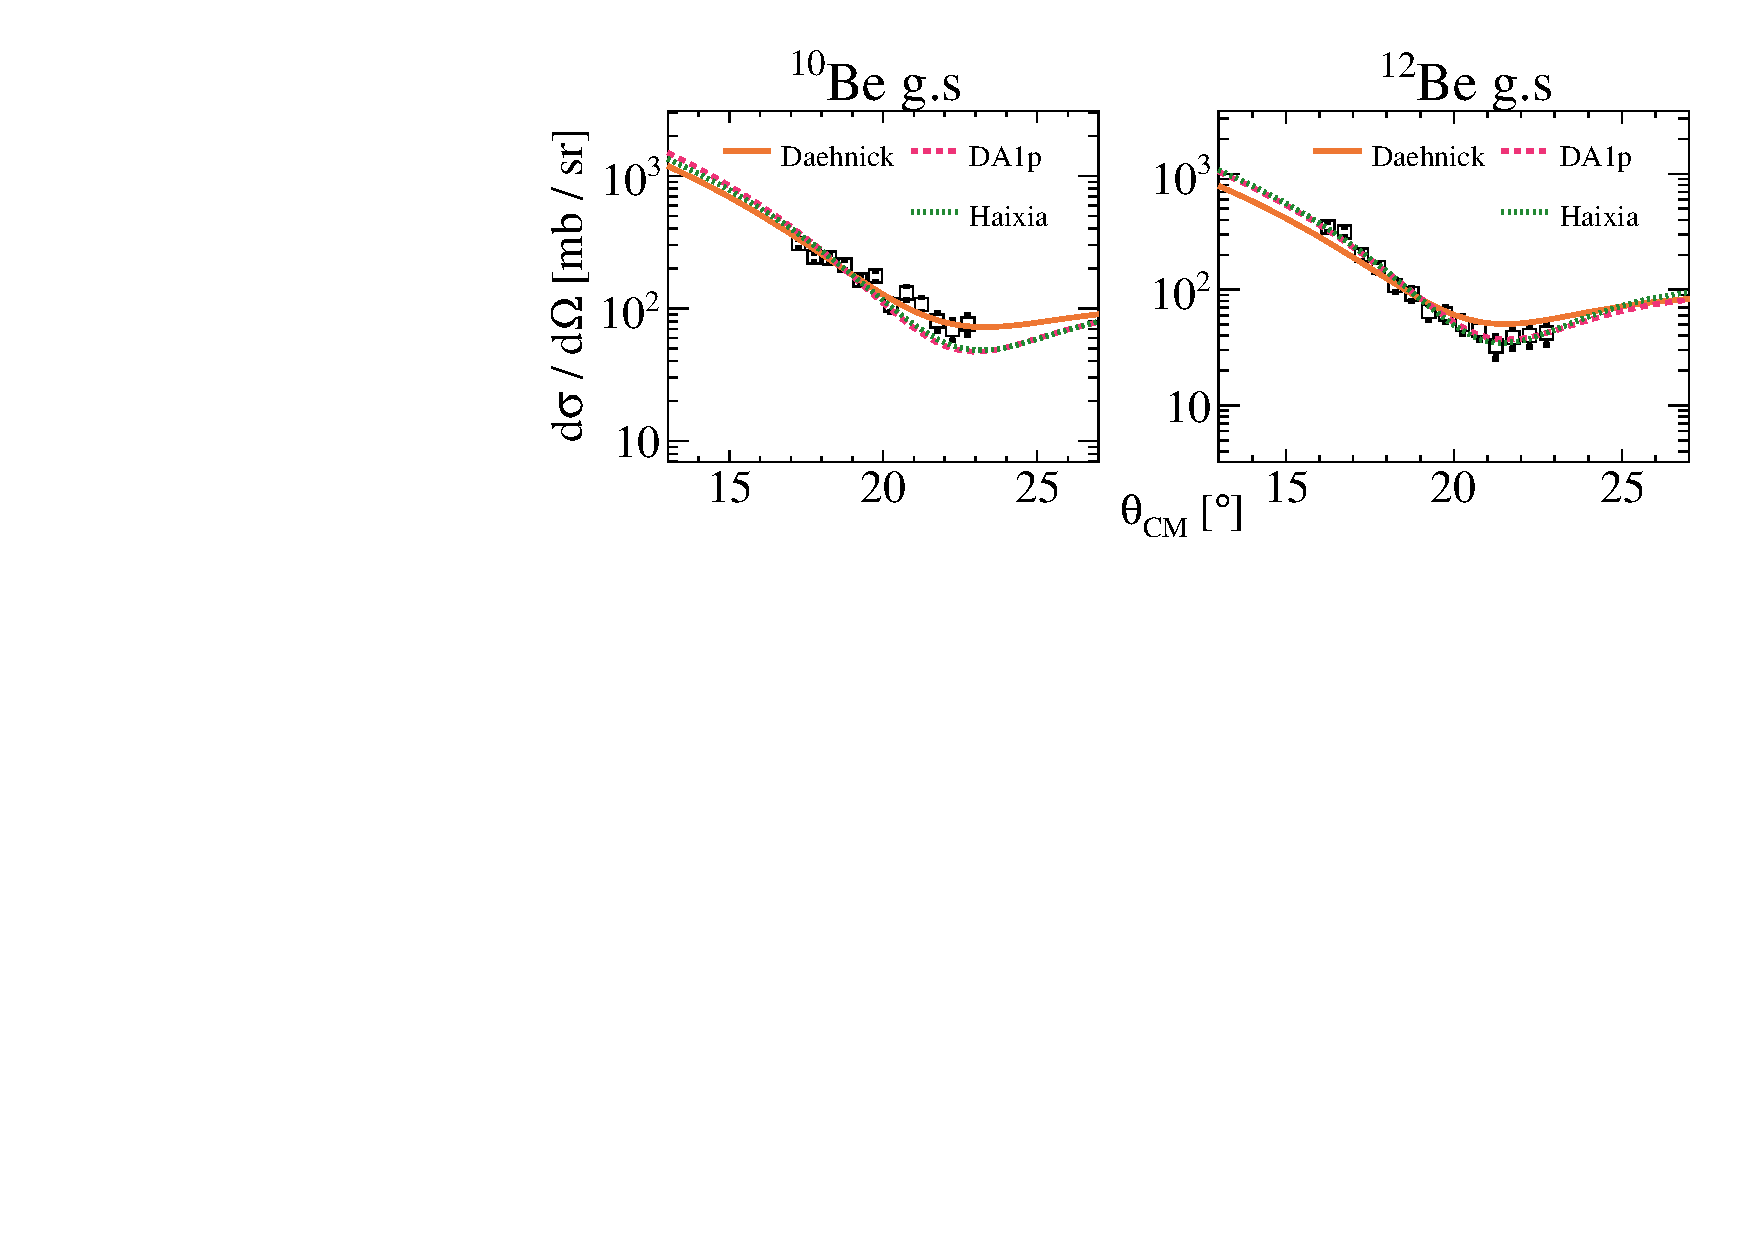
\includegraphics[width=1\linewidth]{figures/elastic.pdf}
        \end{figure}
        \begin{columns}
            \begin{column}{0.5\linewidth}
                \mycolorbox{box2}{
                \iso{10}{Be} + d: \textbf{Daehnick}\\
                {\scriptsize\itshape W. Daehnick et al. PRC 21 (1980)}
                }
            \end{column}%
            \begin{column}{0.5\linewidth}
                \mycolorbox{box4}{
                \iso{12}{Be} + d: \textbf{Haixia}\\
                {\scriptsize\itshape H. Ann, C. Cai. PRC 73 (2006)}
                }
            \end{column}
        \end{columns}
    }
\end{frame}

\begin{frame}[t]{Results: transfer}
    \only<+>{
        The \textbf{ground states} of the heavy recoils are populated.
        \begin{figure}
            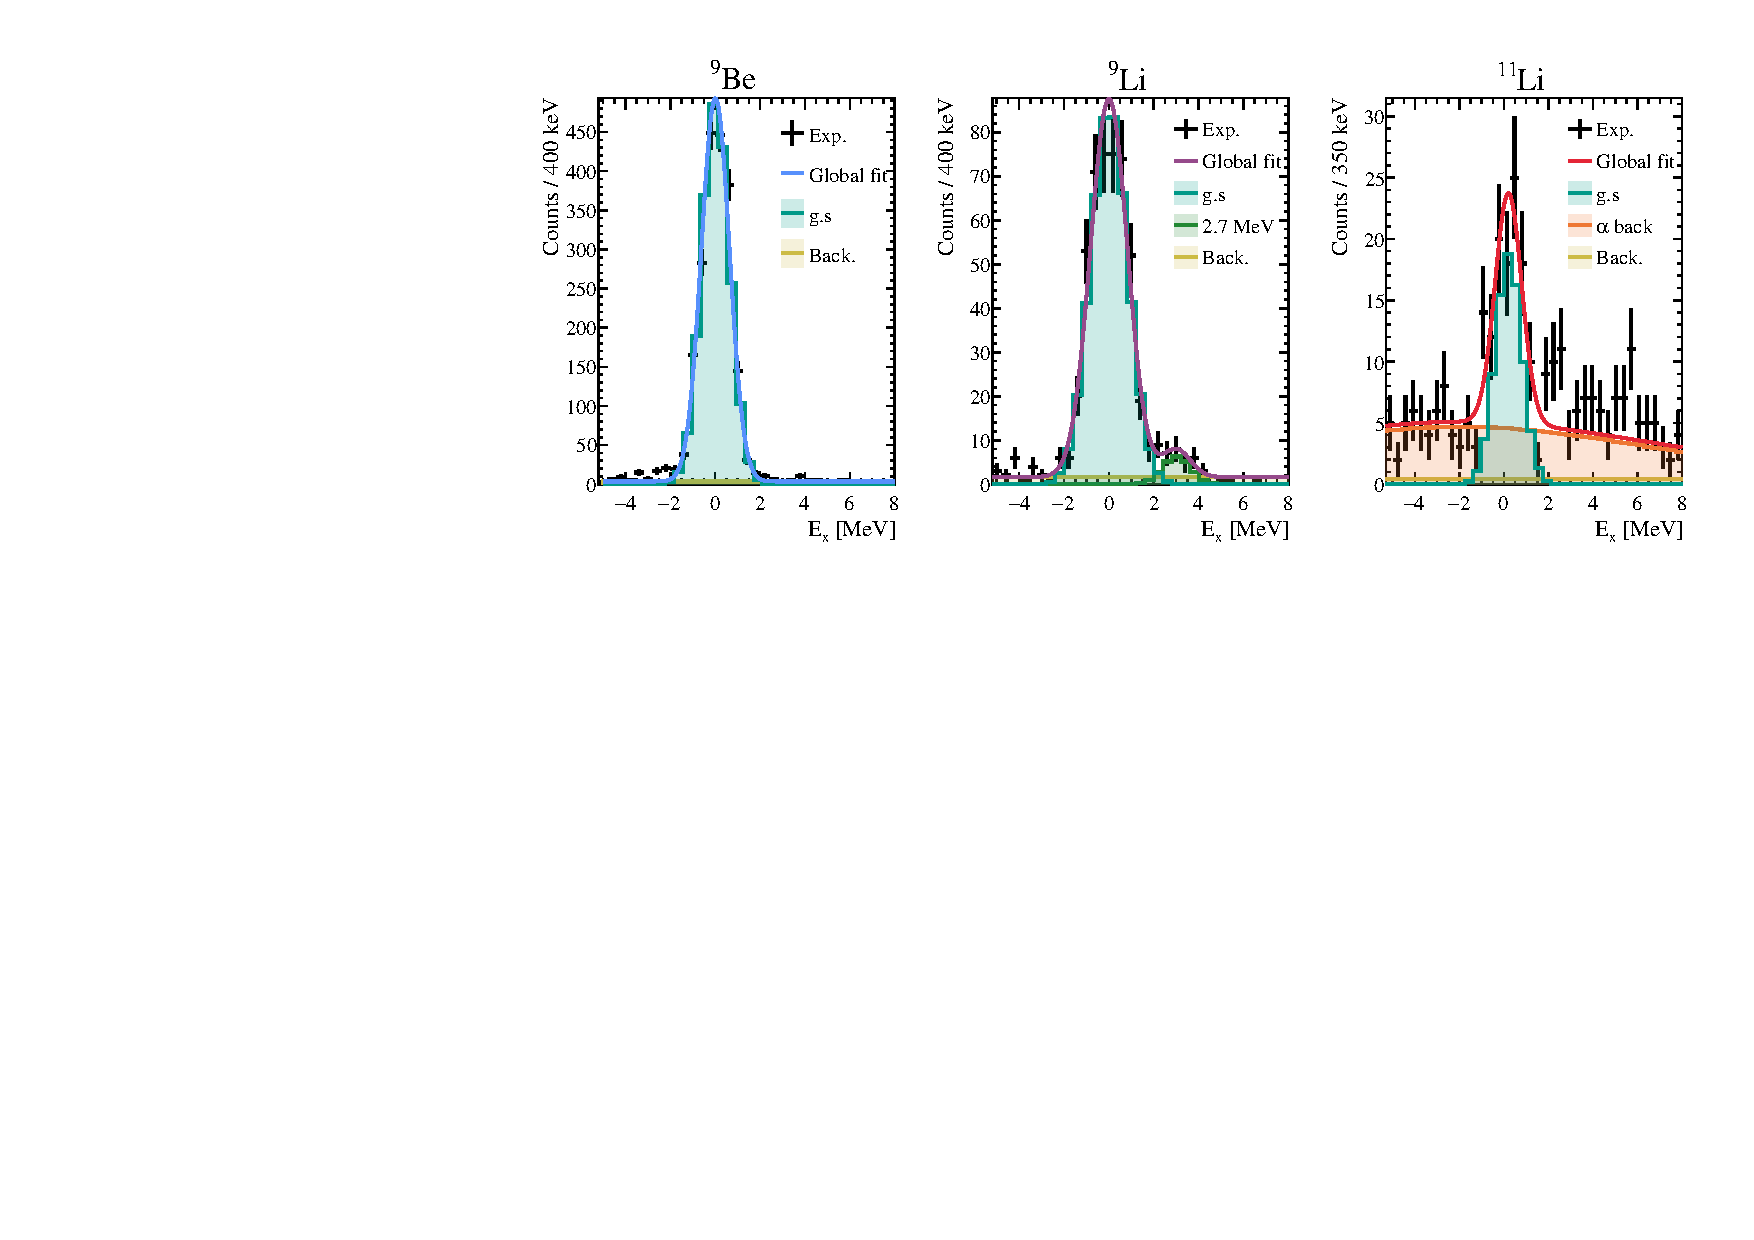
\includegraphics[width=1\linewidth]{figures/transfer_ex.pdf}
        \end{figure}
        \mycolorbox{box2}{
            \textbf{First} state at \qty{2.7}{\MeV} of \iso{9}{Li} is seen too! \emoji{slightly-smiling-face}
        }
    }%
    \only<+>{
        
\includegraphics[height=1.75em]{figures/Fresco2.png} is employed to
        perform the \textbf{DWBA} calculations.
        \begin{columns}[T]
            \begin{column}{0.48\linewidth}
                \mycolorbox[1]{box1}{%
                    \small
                    \textbf{OMP}
                    \begin{itemize}
                        \item In: set from elastic
                        \item Out: HT1p\\
                              {\scriptsize\itshape D. Y. Pang et al., PRC 91 (2015)}
                    \end{itemize}
                }
                \vspace{-1em}
                \mycolorbox[1]{box3}{%
                \small
                \textbf{Light overlap} \\
                {\small $\langle\iso{}{t},\iso{3}{He}\vert\iso{}{d}\otimes \text{n,p}\rangle$}\\
                \vspace{0.5em}
                Accurate GFMC\\
                {\scriptsize\itshape I. Brida et al., PRC 84 (2011)}
                }%
            \end{column}\hfill
            \begin{column}{0.48\linewidth}
                \mycolorbox[1]{box2}
                {
                \boxitem{1} \textbf{Heavy overlap}\\
                {\small$\langle\iso{10,12}{Be}\vert\iso{9,11}{Be,Li}\otimes\iso{}{n,p}\rangle$}\\
                \vspace{0.5em}
                A standard WS\\
                $r_{0} = \qty{1.25}{\femto\m}$, $a = \qty{0.65}{\femto\m}$
                }
                \vspace{-1em}
                \mycolorbox[1]{box4}
                {
                \boxitem{2} \textbf{Heavy overlap}\\
                {\small$\langle\iso{10,12}{Be}\vert\iso{9,11}{Be,Li}\otimes\iso{}{n,p}\rangle$}\\
                \vspace{0.5em}
                WS from novel \textit{Source Term Approach} (STA)\\
                {\itshape\scriptsize N. Timofeyuk PRC 81 (2010)}
                }
            \end{column}
        \end{columns}
    }
\end{frame}

\begin{frame}[t]{Results: transfer}
    Angular distributions for all the states
    \begin{figure}
        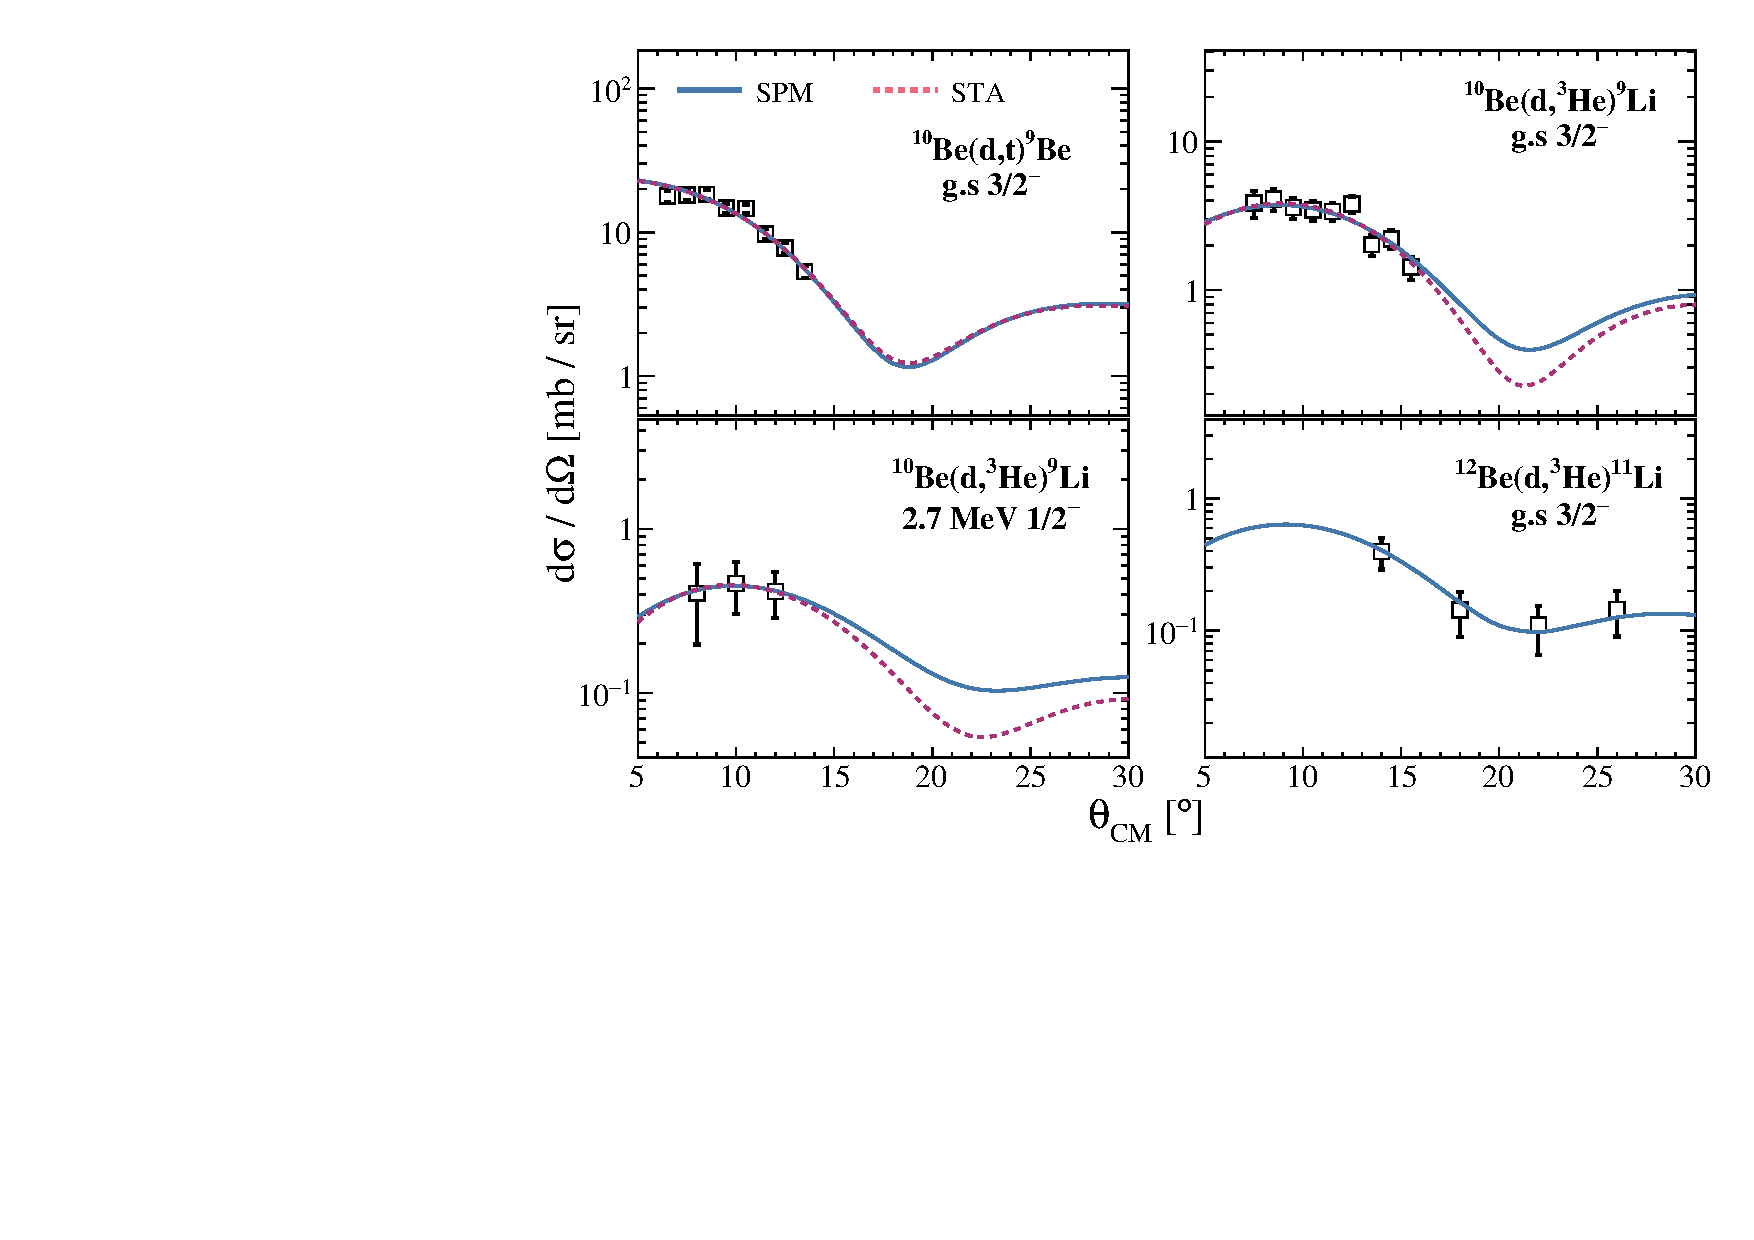
\includegraphics[width=0.85\linewidth]{figures/all_xs.pdf}
    \end{figure}
\end{frame}


\begin{frame}[t]{Results: quenching factor}
    The reduction factor $\text{R}_{\text{S}} = C^{2}S_{\text{exp}} / C^{2}S_{\text{theo}}$ is computed:
    \begin{figure}
        \begin{tikzpicture}
            \node[anchor = south west, inner sep = 0] (image) at (0, 0){
                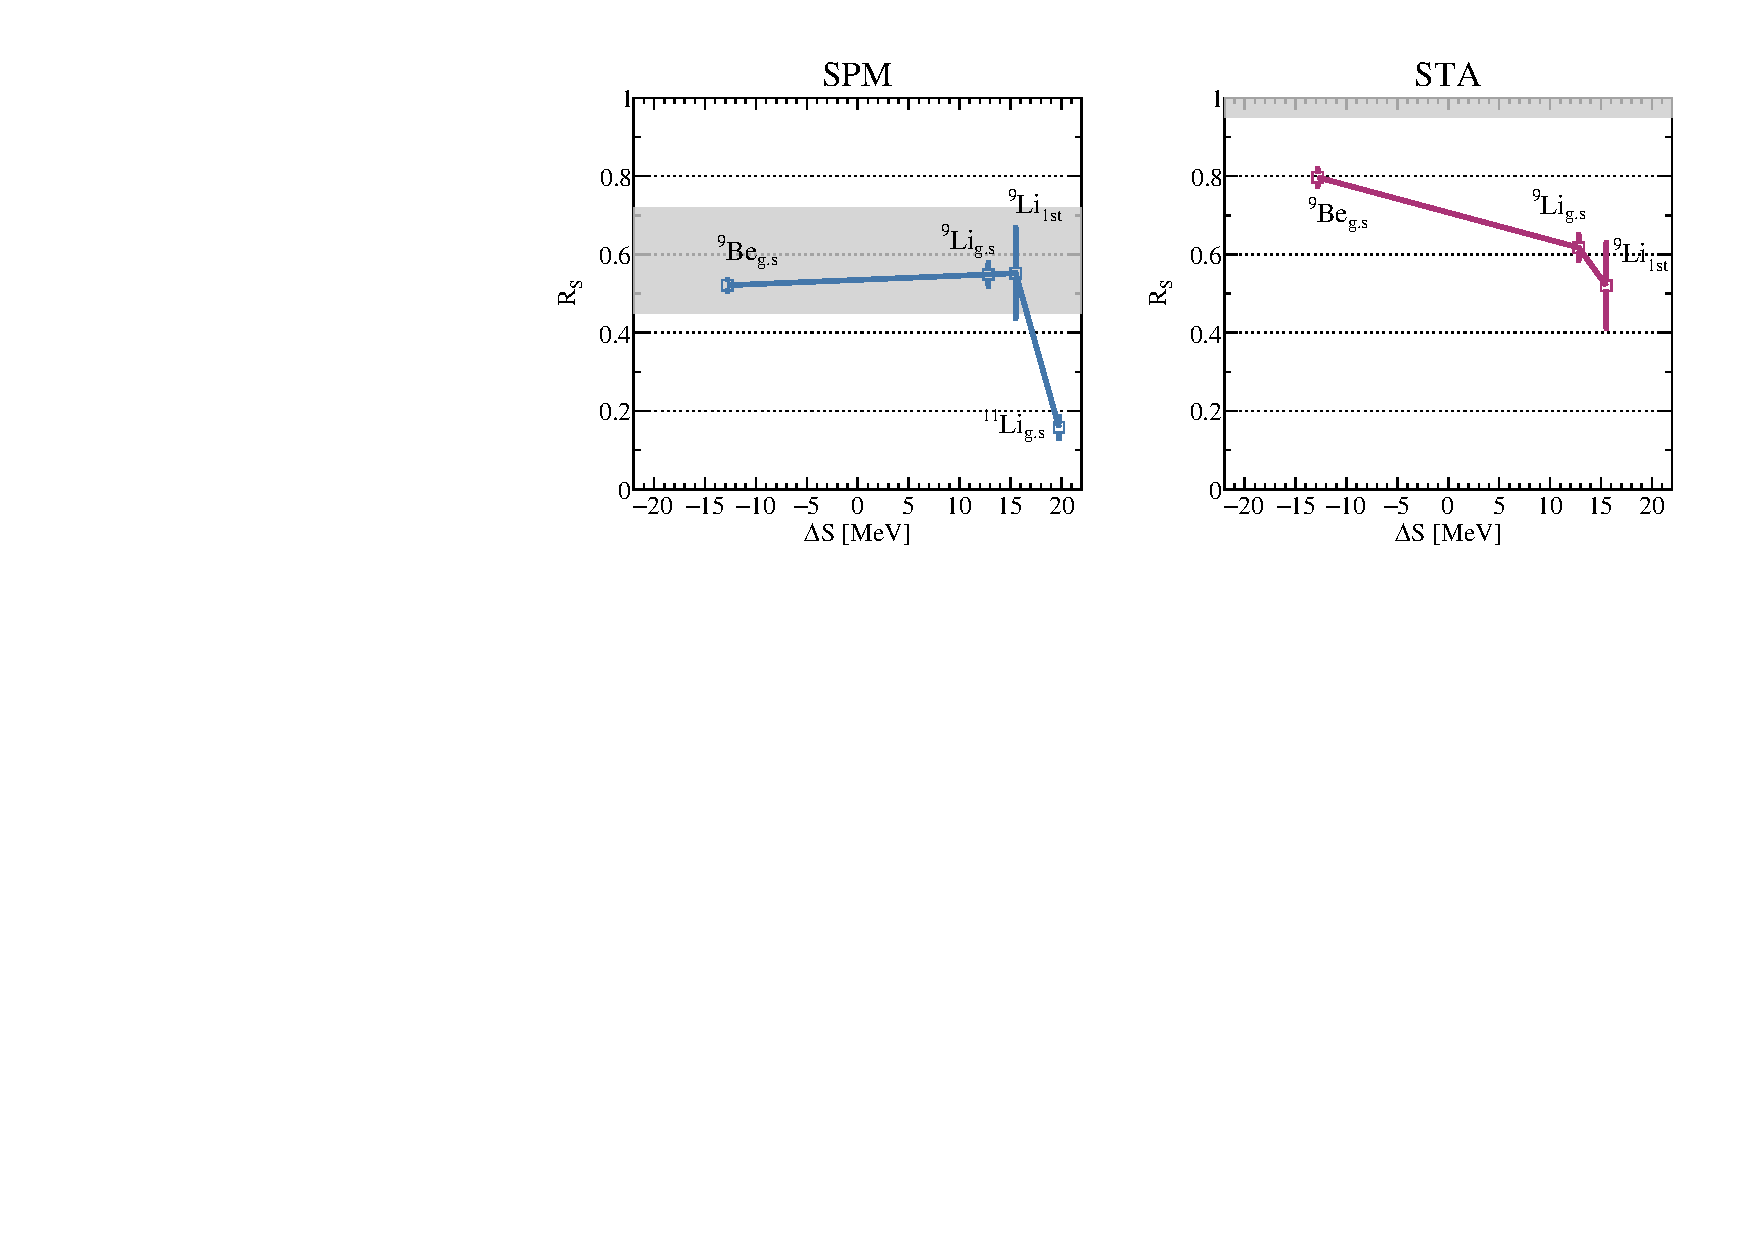
\includegraphics[width=0.9\linewidth]{figures/rs.pdf}
            };
            \only<1>{
                \myscope[false]{
                    \draw[blue1, ultra thick] (0,0) rectangle (0.5,1);
                    \fill [draw=none, fill=white, fill opacity=0.7] (0.51, 0) rectangle (1, 1);
                }}
            \only<2>{
                \myscope[false]{
                    \draw[pink1, ultra thick] (0.5,0) rectangle (1,1);
                    \fill [draw=none, fill=white, fill opacity=0.7] (0, 0) rectangle (0.47, 1);
                }}
        \end{tikzpicture}
    \end{figure}
    \begin{columns}[c]
        \begin{column}{0.33\linewidth}
            \only<1>{
            \mycolorbox[0.95]{box3}{
            \textbf{SFO-tls} interaction\\
            {\itshape\scriptsize T. Suzuki, T. Otsuka PRC 78 (2008)}
            }}%
            \only<2>{
                \mycolorbox[0.95]{box1}{
                    \rs$= 1$\\
                     is expected now
                }}
        \end{column}\hfill
        \begin{column}{0.33\linewidth}
            \only<1>{
                \mycolorbox[0.95]{box4}{
                    \textbf{Compatible} with current systematics \emoji{thumbs-up}
                }}
            \only<2>{
                \mycolorbox[0.95]{box4}{
                    \textbf{Falls short} in modelling SRCs
                }}
        \end{column}\hfill
        \begin{column}{0.33\linewidth}
            \only<1>{
                \mycolorbox[0.95]{box2}
                {
                    \textbf{\iso{11}{Li}} requires GMF correction\\
                    (pending)
                }}
            \only<2>{
                \mycolorbox[0.95]{box2}
                {
                    Needs to be extended to \iso{11}{Li}
                }}
        \end{column}
    \end{columns}
\end{frame}

\begin{frame}[c]{Conclusions}
    \mycolorbox{box3}{
        Angular distributions for \iso{9}{Be}, \iso{9}{Li} and \iso{11}{Li} have been extracted and compared with DWBA
    }
    \vspace{1em}

    \mycolorbox{box2}{
        \rs for SM agrees with literature, while STA still understimates NN correlations
    }
    \vspace{1em}

    \mycolorbox{box1}{
        \iso{11}{Li} needs correction for a major geometrical mismatch value
    }
    \vspace{1em}

    \mycolorbox{box4}{
        STA requires further developments to reach \iso{11}{Li}
    }%
\end{frame}

\begin{frame}[plain]{Acknowledgments}
    \begin{columns}[T]
        \begin{column}{0.33\linewidth}
            The E748 collaboration:
            \begin{itemize}\scriptsize
                \item Santiago:\\
                      B. Fernández
                \item LPC-Caen:\\
                      A. Matta\\
                      F. Delaunay\\
                      N. L. Achouri\\
                      F. Flavigny\\
                      J. Gibelin\\
                      M. Marques\\
                      N. Orr
                \item IJCLab:\\
                      D. Beaumel\\
                      M. Assié\\
                      Y. Blumenfeld\\
                      S. Franchoo\\
                      A. Georgiadou\\
                      V. Girard-Alcindor\\
                      F. Hammache\\
                      N. de Séreville\\
                      A. Meyer\\
                      I. Stefan
            \end{itemize}
        \end{column}
        \begin{column}{0.33\linewidth}
            \begin{itemize}\scriptsize
                \item GANIL:\\
                      B. Jacquot\\
                      O. Kamalou\\
                      A. Lemasson\\
                      M. Rejmund\\
                      T. Roger\\
                      O. Sorlin\\
                      J.C. Thomas\\
                      M. Vandebrouck\\
                      B. Bastin\\
                      F. de Oliveira\\
                      C. Stodel
                \item RIKEN:\\
                      S. Koyama\\
                      D. Suzuki
                \item Surrey:\\
                      N. Timofeyuk
            \end{itemize}

        \end{column}
        \begin{column}{0.33\linewidth}
            
\includegraphics[width=0.6\linewidth]{logos/usc_blue.png}\vspace{1em}
            
\includegraphics[width=0.6\linewidth]{logos/lpc.png}\vspace{1em}
            
\includegraphics[width=0.6\linewidth]{logos/ganil.png}\vspace{1em}
            
\includegraphics[width=0.6\linewidth]{logos/ijclab.png}\vspace{1em}
            
\includegraphics[width=0.6\linewidth]{logos/riken.png}\vspace{1em}
            
\includegraphics[width=0.6\linewidth]{logos/surrey.png}\vspace{1em}
        \end{column}
    \end{columns}
\end{frame}

\begin{frame}[noframenumbering, plain]
    \begin{tikzpicture}[remember picture, overlay]
        \node at (current page.center) {
            \usebeamerfont{frame title}
            \textcolor{mainBlue}{Backup}
        };
    \end{tikzpicture}
\end{frame}


\begin{frame}[t, noframenumbering]{Status with light isotopes}
    Several experiments allowed for the extraction of $C^{2}S$ with Li-induced (d, \iso{3}{He}) reactions:
    \vspace{-1.75em}
    \begin{columns}[c]
        \column{0.48\linewidth}{
            \begin{tikzpicture}
                \node[anchor=south west, inner sep=0](image) at (0,0){
                    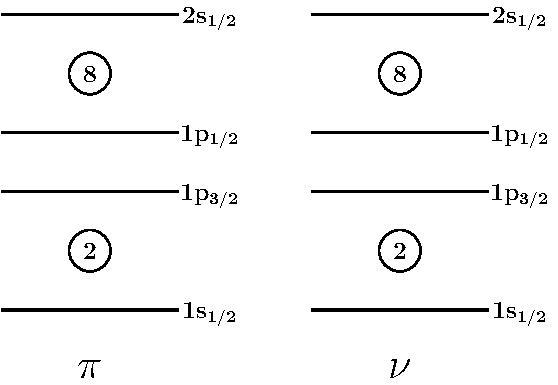
\includegraphics[width=0.75\linewidth]{figures/empty_shell_model.pdf}
                };
                \myscope[false]{
                \node[rectangle, draw, thick, magenta,
                minimum width=1.8cm, minimum height=1.25cm,
                label={[align=center, mainBlue]west:{\small Explored\\ \small region}}] at (0.22, 0.35) {};
                }
            \end{tikzpicture}
        }%
        \column{0.48\linewidth}{
            \begin{figure}
                \begin{tikzpicture}
                    \node[anchor=south west, inner sep=0](image) at (0,0){
                        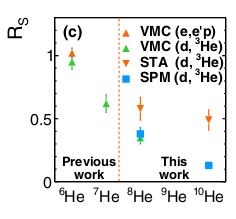
\includegraphics[width=0.75\linewidth]{figures/matta_Rs_Li_He.png}
                    };
                    \myscope[false]{
                    \node[rectangle, draw, very thick, magenta, fit={(0.9, 0.1)(0.8, 0.2)},pin={[mainBlue, pin distance=7mm,
                            pin edge={<-, very thick, black}]75:{\small Unbound!}}
                    ] at (0.9, 0.1) {};
                    }
                \end{tikzpicture}
                \caption{A. Matta \textit{et al.}, Phys. Rev. C 92 (2015)}
            \end{figure}
        }
    \end{columns}
    Several challenges in this region:
    \begin{columns}[T]
        \begin{column}{0.48\linewidth}
            \mycolorbox[0.95]{box3}{
                \enumitem{1} Dealing with \textbf{unbound} nuclei (\iso{10}{He})}
        \end{column}
        \begin{column}{0.48\linewidth}
            \mycolorbox[0.95]{box2}{
                \enumitem{2} Many-body dynamics and/or core excitations}
        \end{column}
    \end{columns}
\end{frame}

\begin{frame}[noframenumbering]{What happens with \texorpdfstring{\iso{11}{Be}}{11Be}?}
    It shows a strong inhibition of the ground state.
    \begin{figure}
        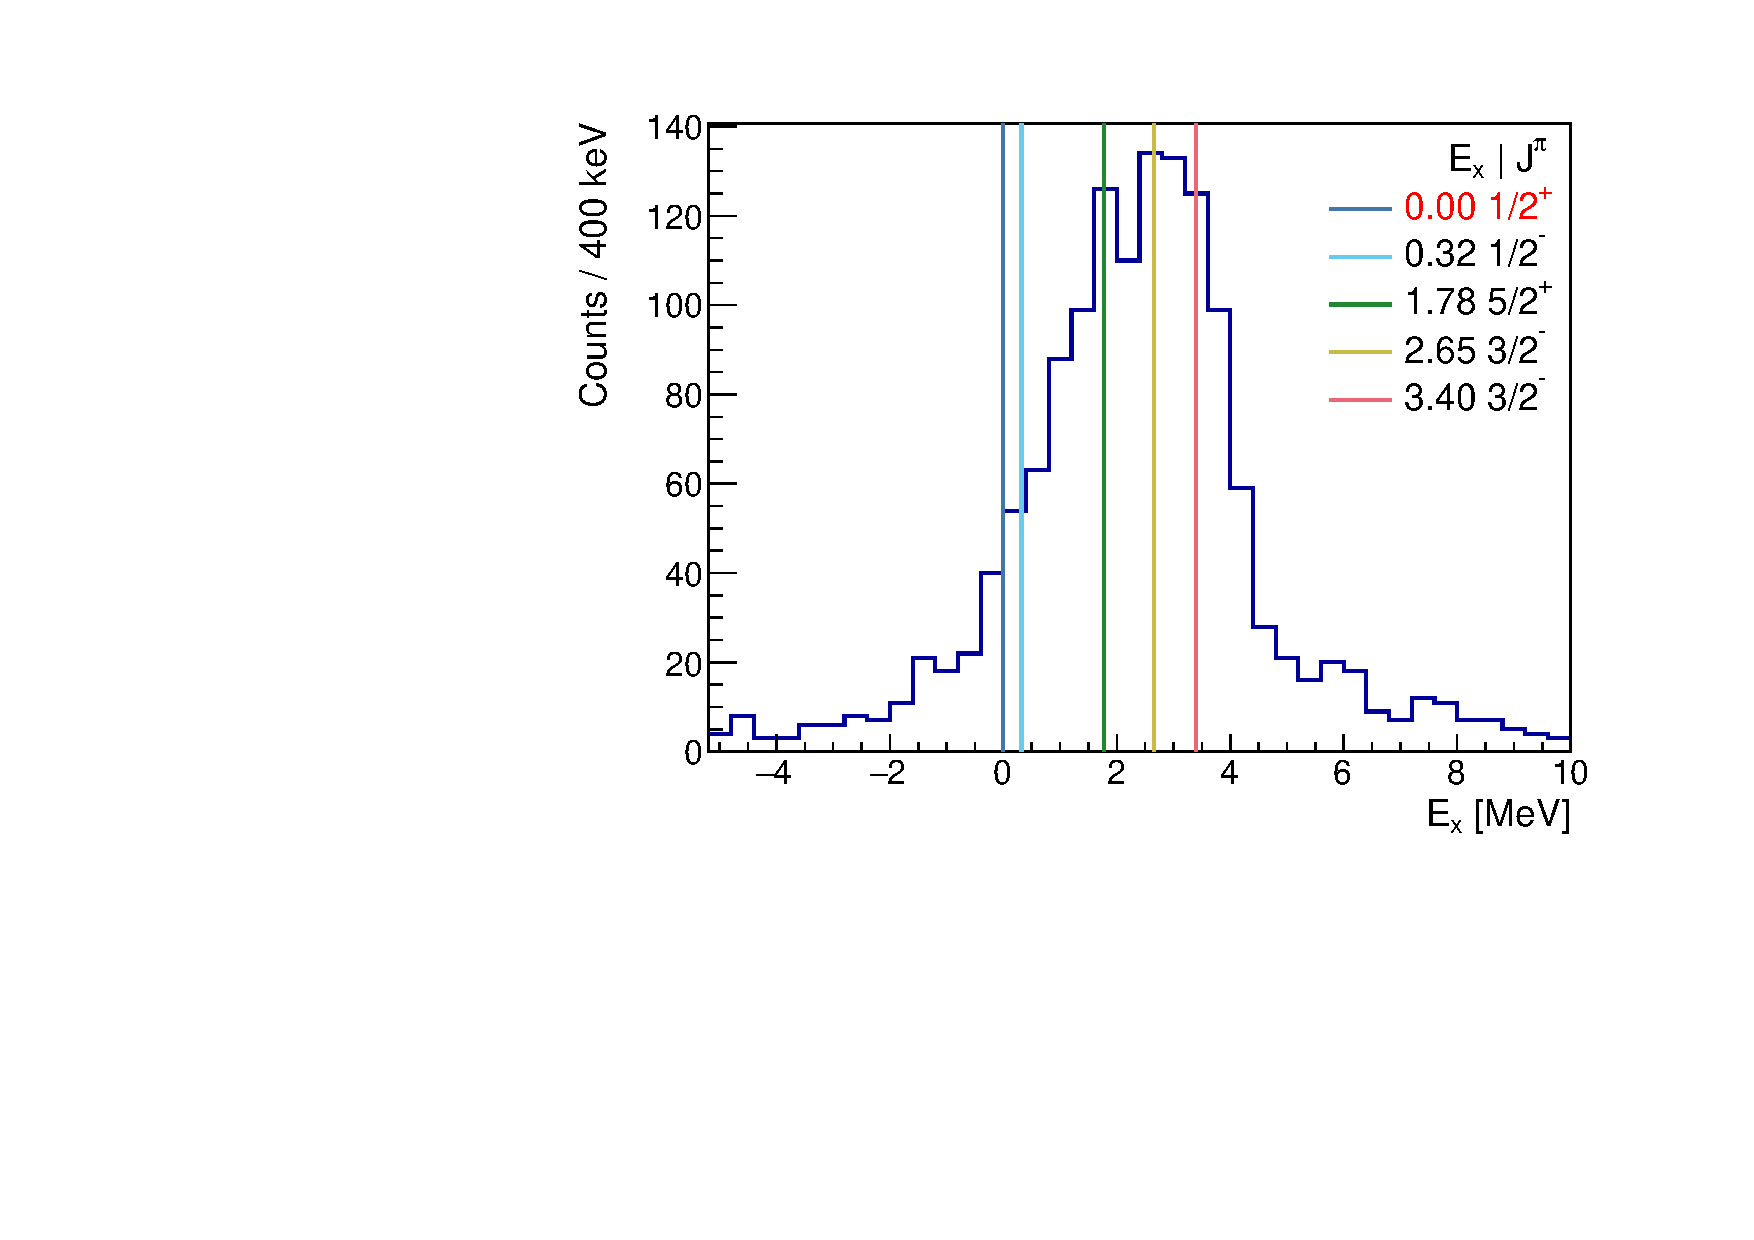
\includegraphics[width=0.8\linewidth]{figures/12Be_dt_ex.pdf}
    \end{figure}
    \mycolorbox{box4}{
        Impossible to disentangle excited states \emoji{frowning-face}
    }
\end{frame}

\begin{frame}[t, noframenumbering]{Results: \texorpdfstring{\iso{10}{Be}(d,\iso{}{t})\iso{9}{Be} }{10Be(d,t)9Be}}
    \begin{figure}
        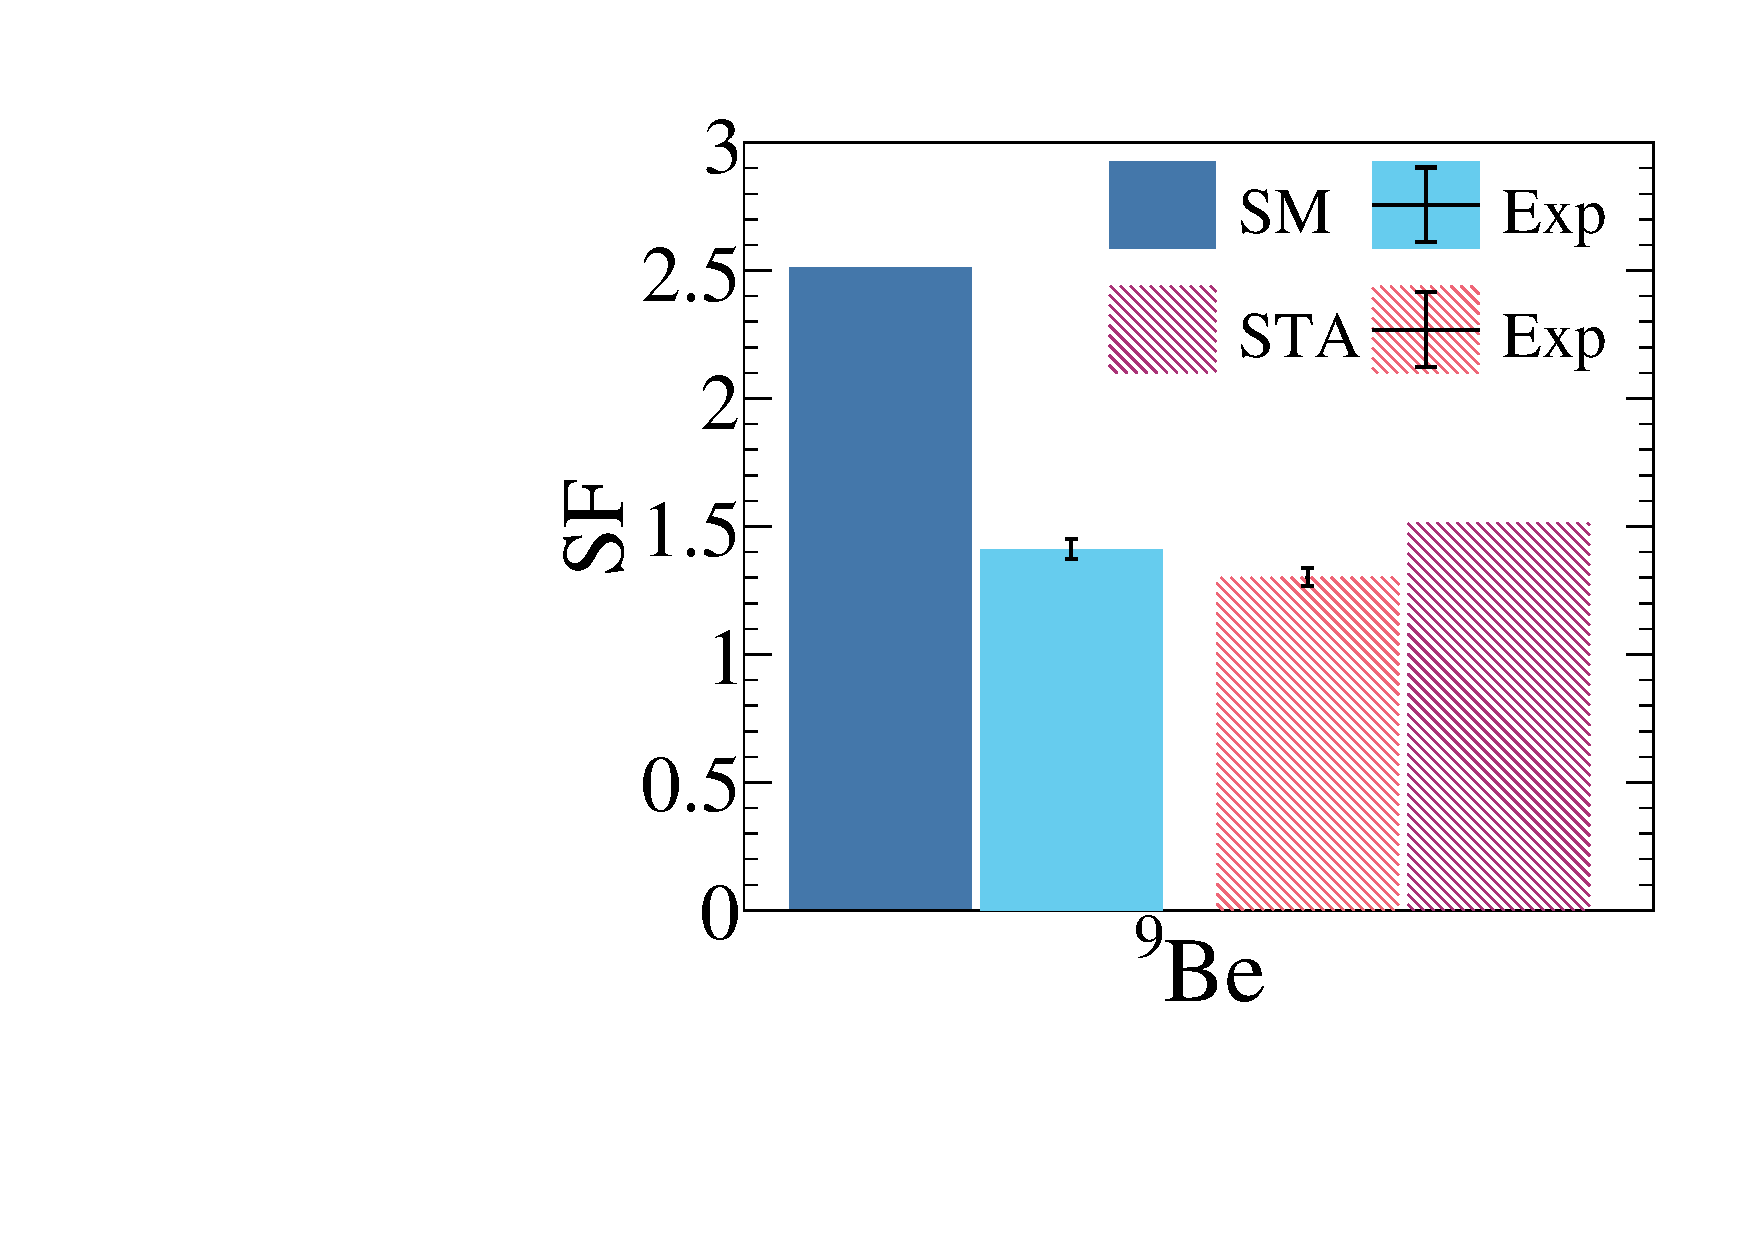
\includegraphics[width=0.5\linewidth]{figures/sf0.pdf}
    \end{figure}
    \begin{columns}[c]
        \begin{column}{0.48\linewidth}
            \mycolorbox[1]{box3}{
            SM calculation using \textbf{SFO-tls} interaction\\
            {\itshape\scriptsize T. Suzuki, T. Otsuka PRC 78 (2008)}
            }
        \end{column}\hfill
        \begin{column}{0.48\linewidth}
            \mycolorbox[1]{box1}{
                \textbf{STA} yields \qty{40}{\percent} of SM value.\\
                Better accord with exp values
            }
        \end{column}
    \end{columns}
\end{frame}

\begin{frame}[t, noframenumbering]{Results: \texorpdfstring{\iso{10}{Be}(d,\iso{3}{He})\iso{9}{Li} }{10Be(d,3He)9Li}}
    \begin{figure}
        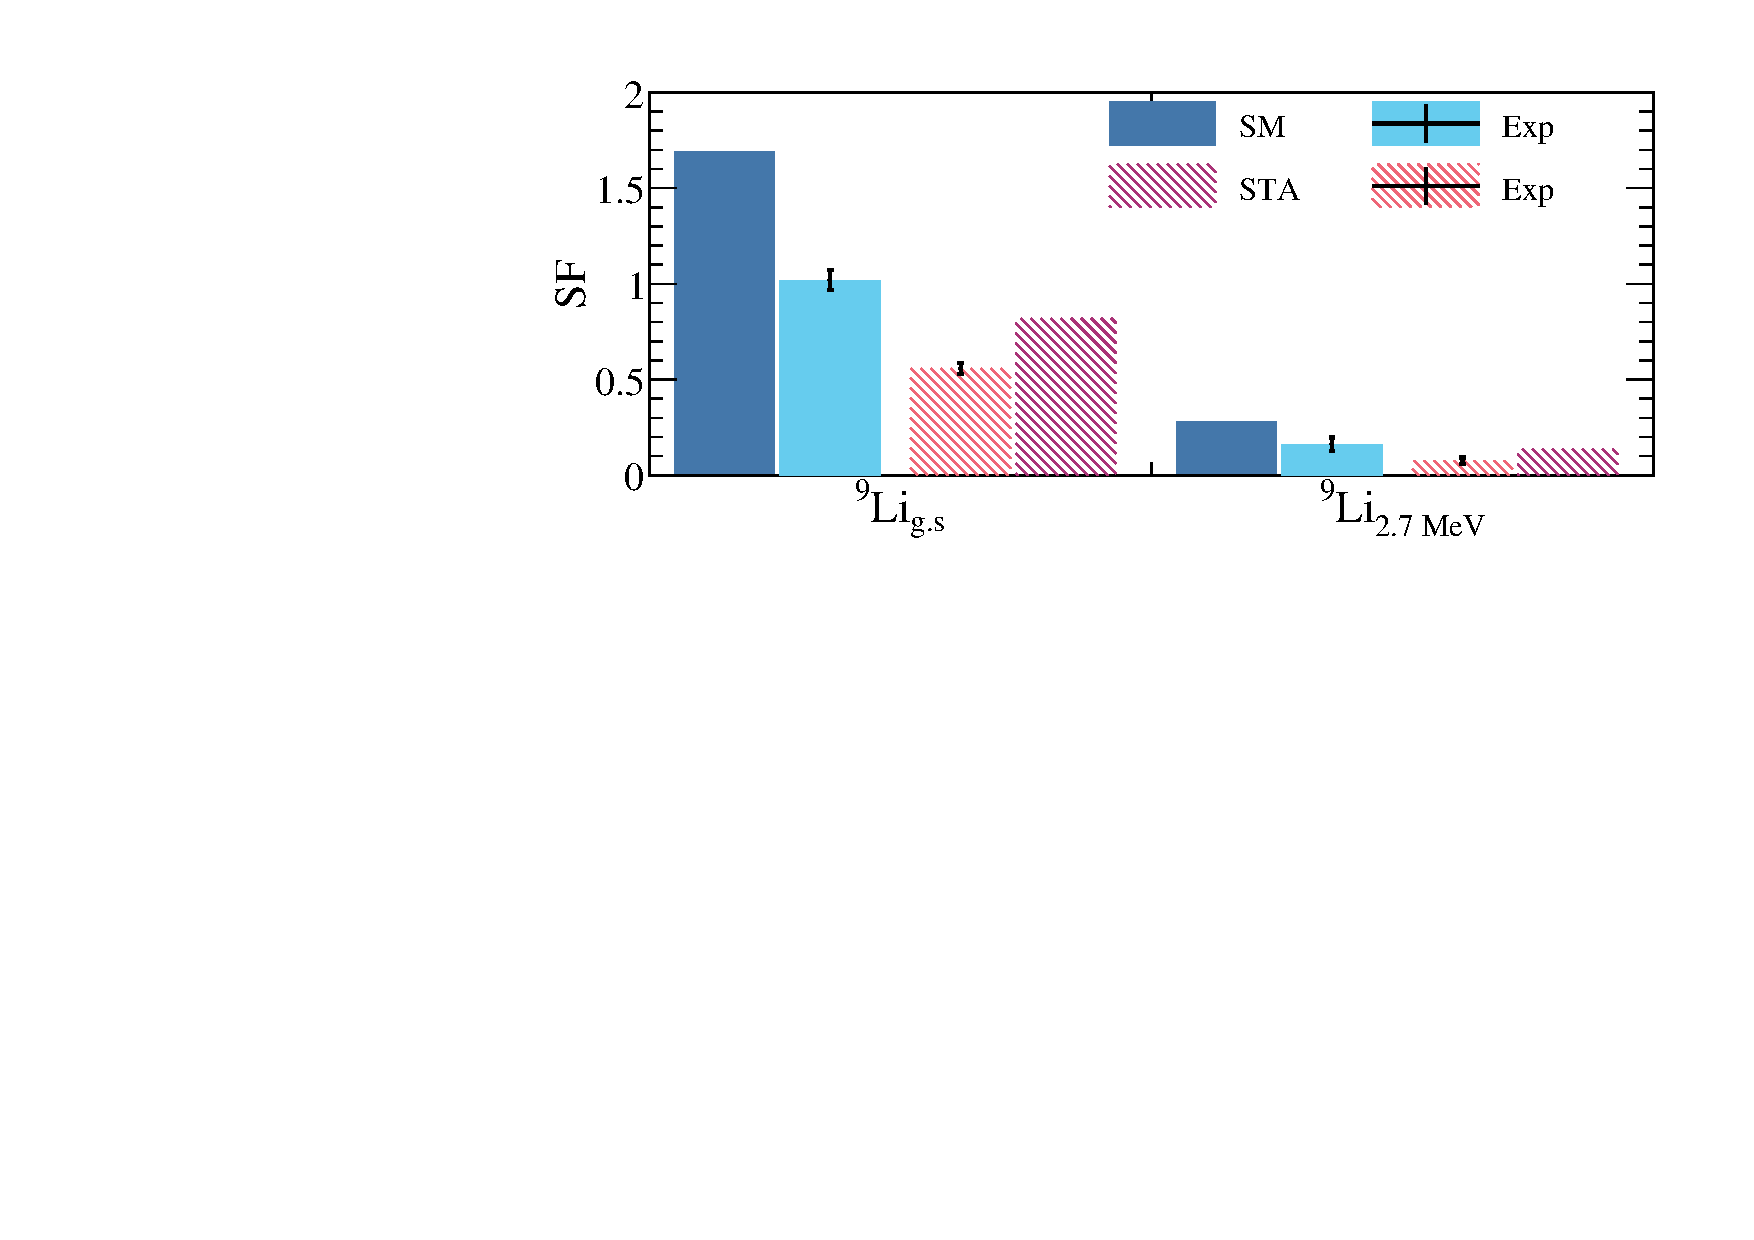
\includegraphics[width=0.9\linewidth]{figures/sf1.pdf}
    \end{figure}
    \begin{columns}[c]
        \begin{column}{0.48\linewidth}
            \mycolorbox[1]{box3}{
                Same significant differences SM-STA
            }
        \end{column}\hfill
        \begin{column}{0.48\linewidth}
            \mycolorbox[1]{box1}{
                Worse agreement within STA data\\
                $\sim$ \qty{40}{\percent} discrepancies
            }
        \end{column}
    \end{columns}
\end{frame}

\begin{frame}[t, noframenumbering]{Results: \texorpdfstring{\iso{12}{Be}(d,\iso{3}{He})\iso{11}{Li} }{12Be(d,3He)11Li}}
    \begin{figure}
        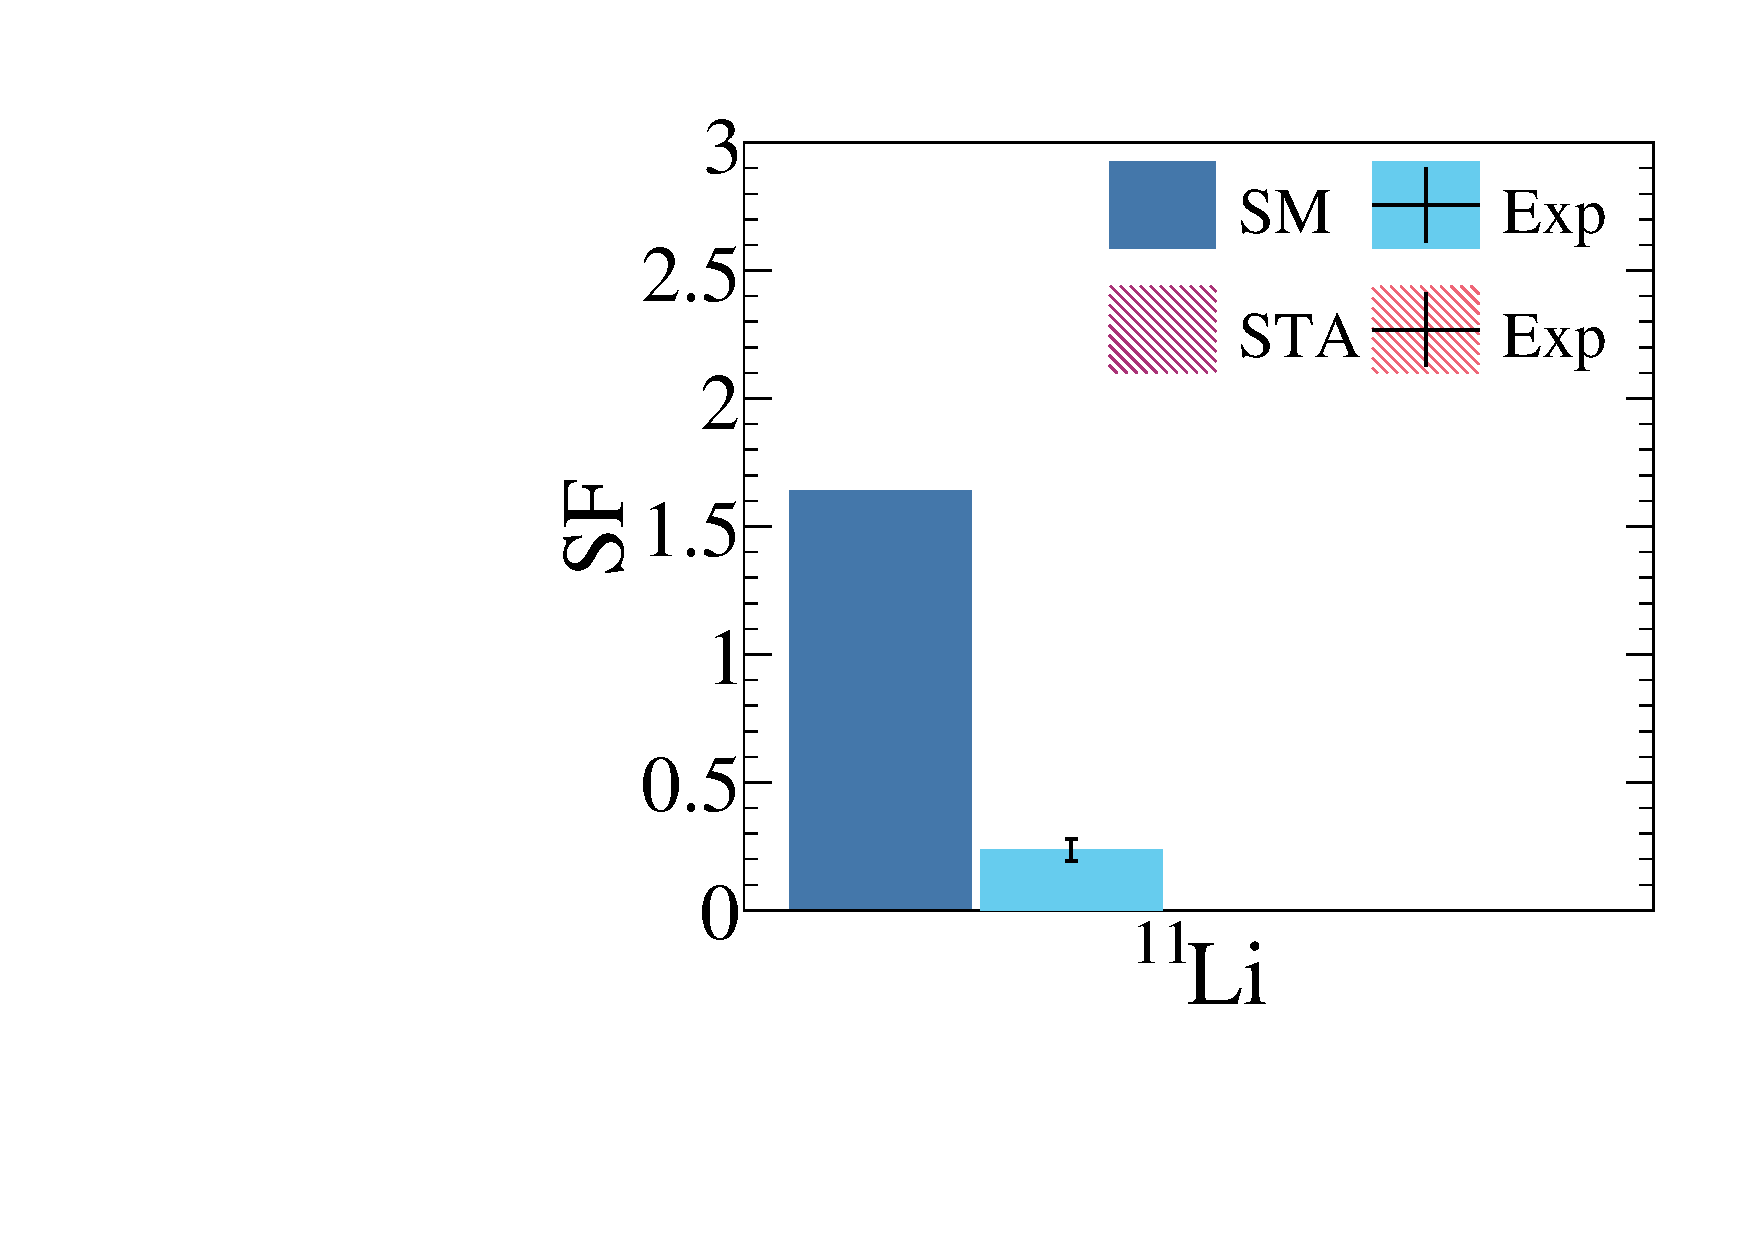
\includegraphics[width=0.5\linewidth]{figures/sf2.pdf}
    \end{figure}
    \begin{columns}[c]
        \begin{column}{0.48\linewidth}
            \mycolorbox[1]{box3}{
                Gigantic quenching, signature of \textbf{GMF} playing a role
            }
        \end{column}\hfill
        \begin{column}{0.48\linewidth}
            \mycolorbox[1]{box1}{
                No STA predictions yet \emoji{confused-face}\\
            }
        \end{column}
    \end{columns}
\end{frame}

\begin{frame}[noframenumbering]{Kinematical lines}
    \begin{columns}[T]
        \begin{column}{0.5\linewidth}
            \begin{tikzpicture}
                \node[anchor=south west, inner sep=0pt] (image) at(0, 0){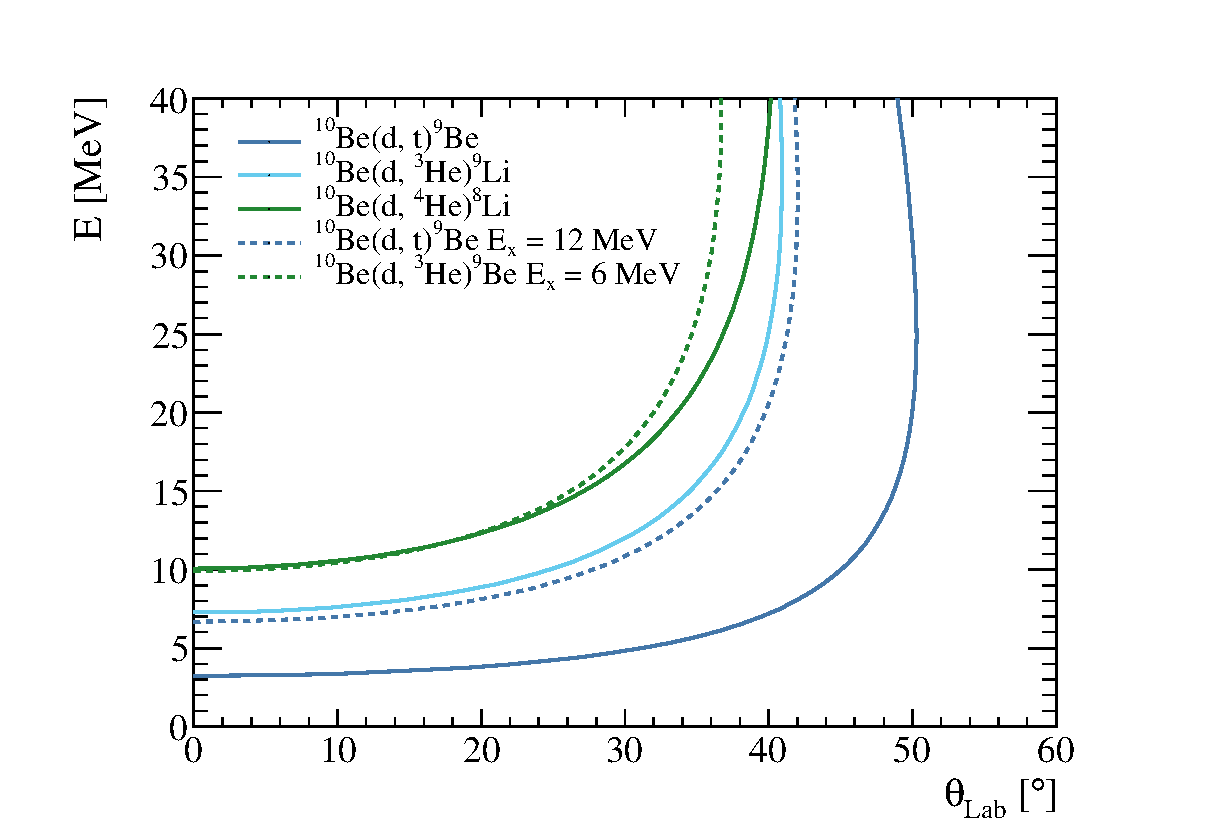
\includegraphics[width=1\linewidth]{figures/kin_10Be.eps}};
                \myscope[false]{
                    \node at (image.north) {\iso{10}{Be}};
                }
            \end{tikzpicture}
        \end{column}
        \begin{column}{0.5\linewidth}
            \begin{tikzpicture}
                \node[anchor=south west, inner sep=0pt] (image) at(0, 0){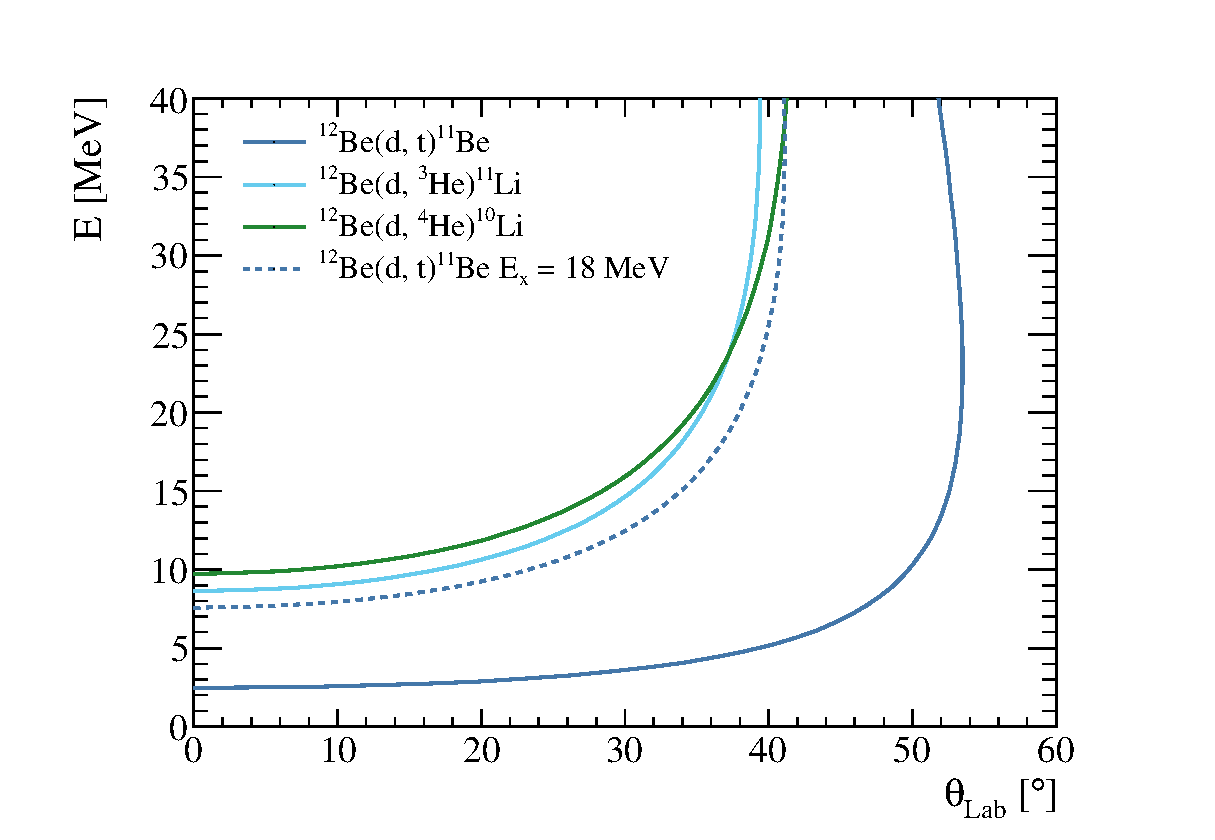
\includegraphics[width=1\linewidth]{figures/kin_12Be.eps}};
                \myscope[false]{
                    \node at (image.north) {\iso{12}{Be}};
                }
            \end{tikzpicture}
        \end{column}
    \end{columns}
\end{frame}

\end{document}